
%\documentclass[preprint,authoryear,12pt]{elsarticle}

%% Use the option review to obtain double line spacing
 %\documentclass[preprint,authoryear,review,12pt]{elsarticle}
%\documentclass[a4paper]{article}
\documentclass[final,authoryear,3p,times,twocolumn]{elsarticle}

\usepackage{geometry}
\geometry{left=3cm,right=3cm,top=3cm,bottom=3cm}
%\renewcommand{\figurename}{Fig.}
%% Use the options 1p,twocolumn; 3p; 3p,twocolumn; 5p; or 5p,twocolumn
%% for a journal layout:
% \documentclass[final,1p,times]{elsarticle}
% \documentclass[final,1p,times,twocolumn]{elsarticle}
%\documentclass[final,3p,times]{elsarticle}
%\documentclass[final,3p,times,twocolumn]{elsarticle}
%\documentclass[final,authoryear,3p,times,twocolumn]{elsarticle}
%\documentclass[final,authoryear,3p,times,twocolumn]{elsarticle}
 %\documentclass[final,5p,times]{elsarticle}
 %\documentclass[final,5p,times,twocolumn]{elsarticle}

%% if you use PostScript figures in your article
%% use the graphics package for simple commands
%% \usepackage{graphics}
%% or use the graphicx package for more complicated commands
%% \usepackage{graphicx}
%% or use the epsfig package if you prefer to use the old commands
%% \usepackage{epsfig}
%\usepackage[thmmarks]{ntheorem}%����֤��
%\usepackage{amsthm}
%\usepackage[fleqn]{amsmath}%�����
%% The amssymb package provides various useful mathematical symbols
\usepackage{amssymb}
\usepackage{nomencl}
%\tolerance=1
%\emergencystretch=\maxdimen
%\hyphenpenalty=10
%\hbadness=10
\usepackage[english]{babel} %%��ֹ���һ����ĸ����
%\usepackage{graphicx}
\usepackage{booktabs}
\usepackage{amsmath,amsthm,amssymb,amsfonts}
\usepackage{color}
\makenomenclature

%% The amsthm package provides extended theorem environments
%% \usepackage{amsthm}

%% The lineno packages adds line numbers. Start line numbering with
%% \begin{linenumbers}, end it with \end{linenumbers}. Or switch it on
%% for the whole article with \linenumbers after \end{frontmatter}.
%% \usepackage{lineno}

%% natbib.sty is loaded by default. However, natbib options can be
%% provided with \biboptions{...} command. Following options are
%% valid:

%%   round  -  round parentheses are used (default)
%%   square -  square brackets are used   [option]
%%   curly  -  curly braces are used      {option}
%%   angle  -  angle brackets are used    <option>
%%   semicolon  -  multiple citations separated by semi-colon
%%   colon  - same as semicolon, an earlier confusion
%%   comma  -  separated by comma
%%   numbers-  selects numerical citations
%%   super  -  numerical citations as superscripts
%%   sort   -  sorts multiple citations according to order in ref. list
%%   sort&compress   -  like sort, but also compresses numerical citations
%%   compress - compresses without sorting
%%
%% \biboptions{comma,round}

% \biboptions{}


%\journal{Ocean }

\begin{document}

\begin{frontmatter}

%% Title, authors and addresses

%% use the tnoteref command within \title for footnotes;
%% use the tnotetext command for the associated footnote;
%% use the fnref command within \author or \address for footnotes;
%% use the fntext command for the associated footnote;
%% use the corref command within \author for corresponding author footnotes;
%% use the cortext command for the associated footnote;
%% use the ead command for the email address,
%% and the form \ead[url] for the home page:
%%
%\title{Title\tnoteref{label1}}
%% \tnotetext[label1]{}
%% \author{Name\corref{cor1}\fnref{label2}}
%%\ead{dittoyiren@gmail.com}
%% \ead{email address}
%% \ead[url]{home page}
%% \fntext[label2]{}
%% \cortext[cor1]{}
%% \address{Address\fnref{label3}}
%% \fntext[label3]{}

\title{Singular perturbations used in rudder roll stabilization of ships on the path following problem}

%% use optional labels to link authors explicitly to addresses:
 \author[1]{RY Ren}
 \author[1,2]{ZJ Zou} \ead{zjzou@sjtu.edu.cn}
 \author[1]{XG Wang}
 \address[1]{School of Naval Architecture,Ocean and Civil Engineering, Shanghai Jiao Tong University, Shanghai 200240, China}
 \address[2]{State Key Laboratory of Ocean Engineering, Shanghai Jiao Tong University, Shanghai 200240, China}

 %\author[label1,label2]{<author name>}
%% \address[label1]{<address>}
%% \address[label2]{<address>}
%
%\author{RY Ren, ZJ Zou, XG Wang}
%
%\address{Shanghai Jiaotong university}
%\printnomenclature
\begin{abstract}
%% Text of abstract
A singular perturbation approach is used to design a control law used in the rudder roll stabilization (RRS) system of ships. Different from most of the existing research on RRS system, which only consider the course keeping problem, in this paper the RRS performance in the path following case is taken into consideration. This problem is challenging mostly due to the complex coupling effects between the roll motion and other Degree-of-Freedoms (DoFs).By introducing the singular perturbation method, the whole system is divided into two time scale subsystems, namely the slow subsystem which describes the surge-sway-yaw motions, and the fast subsystem which describes the roll motion. Coupling effects of the two different time scale subsystems can be easily considered in the analysis framework of singular perturbation. The control laws of the two subsystems thus can be designed separately, which makes the system much simpler. Guidance-based approach is used the analyze and control the slow subsystem, and a mass-spring-damper equation is used to describe the fast roll subsystem. Stability is guaranteed in the designed control laws. Simulation results show the effectiveness and robustness of this approach used in RRS system in Path Following problem.
\end{abstract}

\begin{keyword}
%% keywords here, in the form: keyword \sep keyword
rudder roll stabilization; path following; coupling effects; time scale decomposition; singular perturbation; 
%% MSC codes here, in the form: \MSC code \sep code
%% or \MSC[2008] code \sep code (2000 is the default)

\end{keyword}

\end{frontmatter}

%%
%% Start line numbering here if you want
%%
% \linenumbers

%% main text
\section{Introduction}
Roll motion is considered to be the principal villain to cause the discomfort to the passengers, decrease the work efficiency of the crew, damage the cargo, and in some extreme cases, may cause the capsizing of the ship. Therefore, enforcing roll constraints while maneuvering in seaways is an important issue in surface vessel control community, it has become an active research area since 1970s. Criteria of the maximum roll angle for different work conditions have been made by Faltinsen \citep{faltinsen1993sea}. It is suggested that the maximum root mean square of roll angle should be less than six degrees for light manual work and three degrees for intellectual work. 


In the past decades, many devices have been designed to reduce the roll motion, both active control and passive control devices, such as bilge keels, gyroscopic stabilizers, anti-rolling tanks, stabilizing fins and moving weights \citep{treakle2000time,gawad2001roll,perez2002simulation,townsend2007new,surendran2007studies}. However, all these approaches need extra devices and installation costs, thus are usually expensive. Due to the fact that rudder action can also cause certain roll motion for most surface ships, although the original objective of the rudder is to steer the ship to a desired course, it is expected that if the rudder is suitably operated according to the roll motion and the course deviation, the roll angle may be reduced to some degree, at the same time the heading is not violently changed. This rudder roll stabilization (RRS) control strategy needs no extra devices and is relatively cheap, thus has drawn many researchers' interests in the past decades \citep{van1990rudder,blanke1993rudder,lauvdal1998rudder,perez2005ship}. Model experiments and full-scale trails have been made to evaluate its effectiveness in practice \citep{van1990rudder}. In RRS control system, rudder is the only actuator for two outputs (roll and heading), thus sufficient bandwidth separation of the two loops has to be guaranteed.


Among the previous research, most of the 

There are also several drawbacks of RRS, such as the inefficiency at low speed and severe feedback limitations due to rudder saturation and rate limits. Besides, it is well-known that ships have non-minimum phase (NMP) behavior in the rudder-to-roll dynamics, which is considered to be one major challenge for RRS \citep{lauvdal1997nonlinear,perez2005ship}. NMP systems have an inverse initial response and large phase lag. The NMP behavior in roll motion often causes a fundamental limitation in the RRS system: disturbances attenuation at some frequencies will result in amplification at other frequencies. This limitation thus poses a trade-off between reducing the roll angle at certain frequencies and amplification at others \citep{perez2005ship}.

The NMP phenomenon often arises from the interaction between opposite fast and slow dynamic effects in the system \citep{perez2005ship}. As to the ship, the NMP behavior in roll motion is caused by the fact that the roll dynamics is much faster than the other DOFs. Singular perturbation approach is such a method to analyze and separate the different time scale motions in control problems. In this paper, the RRS system for ships is decomposed into two different time scale subsystems, namely the quasi-steady-state (slow) subsystem and boundary layer (fast) subsystem. The control objectives and control strategies of the two subsystems are treated separately.


%%As to the ship, due to the fact that the inertial moment and added damping moment of roll motion is much smaller than yaw, the roll response is thus much faster than yaw motion. When the rudder is steered, the ship heels to an inward direction at the first stage, because of the roll moment produced by the rudder. While at the next stage, due to the hydrodynamic effects and centrifugal acceleration force, the main heel often changes to an outward direction\citep{oda1996statistical}.

%From frequency domain point of view, enough bandwidth separation is needed for RRS system between rudder-to-roll and rudder-to-yaw motion. Similarly, from time domain point of view, different time-scale motions are necessary to design a single input multiple output (SIMO) control law for the RRS system.

Singular perturbation approaches have been used in aerospace industry for many years as a time-scale separation technique \citep{mehra1979study,bertrand2011hierarchical,esteban2012three}. For example, a three-time scale control law is designed for a nonlinear helicopter model in vertical flight \citep{esteban2012three}. This can be done due to three different time scales of altitude motion, angular velocity, and the associated collective pitch angle of blades. A comprehensive literature review of singular perturbation used in aircraft control was made by Naidu and Calise \citep{naidu2001singular}. However, despite of the extensive work in aerospace industry, few work of singular perturbation and time scale separation techniques has been done in ship control community. This is mainly due to the relatively poor rudder effect and simple control objectives for a ship control system. However, when a RRS problem is considered, the traditional 3-DOF model (surge-sway-yaw) is coupled with fast roll motion, and different time scale motions do exist in this system. The concept of time scale separation based on singular perturbation can be used to analyze such problems in a natural and elegant way.

Singular perturbation is a means of taking into account the often neglected high-frequency phenomena and considering them in a separate fast time scale \citep{kokotovic1987singular}. By introducing a small parameter $\varepsilon$, the fast varying state variables are described in the form of singular ordinary differential equations (ODEs), the equations become singular when $\varepsilon$ tends to zero. A stretched time scale is used to describe the fast dynamics and the slow state variables are regarded to be constant in this time scale. A so-called quasi-steady-state equilibrium (QSSE) is used to pass information between different time scale subsystems.

This paper introduces the singular perturbation approach to analyze the ship RRS problem. There are three major merits of using this approach in RRS system.

Firstly, more detailed analysis is possible in time domain, such as stability issues and time domain response. Unlike traditional analysis methods, whose emphasis is on the bandwidth separation in Bode diagram considered in frequency domain, this paper emphasizes the separation of different time scale subsystems in time domain. The stability and robust analysis are easily conducted in this model, and the sensitivity analysis to model errors can also be evaluated within this framework, which are not easily conducted in frequency domain.

Secondly, the time scale decomposition approach and separate control strategy simplify the control law design for RRS system. By using singular perturbation method, the original underactuated RRS system can be decomposed into two single input single output (SISO) subsystems, thus is relatively easier to obtain the appropriate control law that can stabilize each subsystem.   %In practice, only yaw angle is considered in feedback on course-keeping problem,

Thirdly, the proposed separate control strategy considers the interaction between different time-scale subsystems. The coupling effect is important in some cases, and singular perturbation approach takes this into consideration though QSSE.

%In this paper, a track keeping simulation case with a large initial deviation from the desired path is conducted to evaluate the validity of the designed RRS control law, where the coupling effect may be an issue.}

In this paper, a simplified 3-DOF (sway-roll-yaw) linear model is used to design and analyze the RRS control law. As course keeping operations are considered in most situations, thus the linear model has considerable accuracy in these problems \citep{perez2005ship}. Li et al. \citep{li2009design} used a comprehensive 4-DOF (surge-sway-roll-yaw) nonlinear model as a virtual ship for simulation and performance evaluation. This nonlinear model was obtained by a set of captive model tests \citep{son19825}. It is selected as a benchmark model to evaluate the performance of the linear model in this paper. The different performances between the linear and nonlinear models are evaluated.


The structure of this paper is as follows. Section 2 introduces the nonlinear and linearized models of motion of surface ships, the model of disturbances is also described. Section 3 gives a brief introduction to the singular perturbation approach, based on which the the RRS control is designed. Robustness analysis of the unmodeled dynamics is also made in this section. Section 4 gives the simulation results. Section 5 is the conclusion.

\section{Model definition and analysis}
In this section, the models of ship motion and environmental disturbances are described. %In this paper, linear model is used to analyze the system and design the control law, both the linear and nonlinear model are used to simulation.
\subsection{4-DOF nonlinear model}
A ship in a seaway moves in 6-DOFs. Three translation displacements are used to define the location and three angular displacements are used to define the orientation. These motions are often described in two types of reference frame, namely the inertial frames and body-fixed frames.

As shown in Fig. \ref{FIG1_PDF}, the location and orientation of the ship are described in the inertial frame, the translation displacements and angular displacements are described as $[x_0,y_0,z_0]^T$ and $[\phi,\theta,\psi]^T$, where $x_0,y_0$ and $z_0$ are the three coordinates of the ship, $\phi$, $\theta$ and $\psi$ are roll, pitch and yaw angle, respectively. The components of the force and moment $[X,Y,Z]^T$, $[K,M,N]^T$, the components of the translational velocity and the angular velocity $[u,v,w]^T$, $[p,q,r]^T$, are described in the body-fixed frame, where $u,v$ and $w$ are surge, sway and heave velocity, and $p,q$ and $r$ are roll, pitch and yaw rate, respectively. The rudder angle is expressed as $\delta$.

In traditional maneuvering issues, such as course-keeping problem, normally only a 3-DOF model (surge-sway-yaw) is considered. However, when consider the RRS problem, a 4-DOF model including the roll motion is needed. In this paper, a comprehensive 4-DOF nonlinear model (surge-sway-roll-yaw) is used to describe the RRS system \citep{fossen1994guidance}: %This nonlinear model captures the essential characteristics of the ship dynamics\citep{li2009path}. And also, this container have a relative long nature roll period, which is about 30 second, this kind of ship is more suited to the application of RRS according to \citep{perez2005ship,cowley1974development}, because the roll moments generated by the rudder are not limited by the rates of the steering machinery.
\begin{eqnarray}
(m+m_x)\dot{u}-(m+m_y)vr=X \label{nonli1}\\
(m+m_y)\dot{v}+(m+m_x)ur+m_y\alpha_y\dot{r}-m_yl_y\dot{p}=Y\\
(I_x+J_x)\dot{p}-m_yl_y\dot{v}-m_xl_xur+W\overline{GM}\phi=K\\
(I_z+J_z)\dot{r}+m_y\alpha_y\dot{v}=N-Yx_G\label{nonli4}
\end{eqnarray}
where $m, I_x$ and $I_z$ denote the mass and moment of inertia of the ship. $m_x, m_y,J_z,J_x$ denote the added mass and added moment of inertia in corresponding directions. $W$ is the ship displacement. $\overline{GM}$ is the metacentric height. $l_x$ and $l_y$ denote the $z$-coordinates of the centers of $m_x$ and $m_y$ respectively. $\alpha_y$ denotes the $x$-coordinates of the center of $m_y$. $x_G$ is the $x$ coordinate of the gravity center. $X$, $Y$, $K$ and $N$ are the hydrodynamic forces and moments in corresponding directions, whose detailed expressions in form of hydrodynamic coefficients can refer to Fossen's book \citep{fossen1994guidance}.

%\begin{equation}
%(m+m_x)\dot{u}-(m+m_y)vr=X
%\end{equation}
%
%\begin{equation}
%(m+m_y)\dot{v}+(m+m_x)ur+m_y\alpha_y\dot{r}-m_yl_y\dot{p}=Y
%\end{equation}
%
%\begin{equation}
%(I_x+J_x)\dot{p}-m_yl_y\dot{v}-m_xl_xur+W\overline{GM}\phi=K
%\end{equation}
%
%\begin{equation}
%(I_z+J_z)\dot{r}+m_y\alpha_y\dot{v}=N-Yx_G
%\end{equation}%

%
%\begin{eqnarray}
%X&=&X(u)+(1-t)T(J)+X_{vr}vr+X_{vv}v^2\\
%& &+X_{rr}r^2+X_{\phi\phi}\phi^2+c_{RX}F_Nsin\delta\nonumber
%\end{eqnarray}
%\begin{eqnarray}
%Y&=&Y_vv+Y_rr+Y_pp+Y_{\phi}\phi+Y_{vvv}v^3+Y_{rrr}r^3\\
%& &+Y_{vvr}v^2r+Y_{vrr}vr^2+Y_{vv\phi}v^2\phi+Y_{v\phi\phi}v\phi^2\nonumber\\
%& &+Y_{rr\phi}r^2\phi+Y_{r\phi\phi}r\phi^2+(1+a_H)F_Ncos\delta\nonumber
%\end{eqnarray}
%\begin{eqnarray}
%K&=&K_vv+K_rr+K_pp+K_{\phi}\phi+K_{vvv}v^3+K_{rrr}r^3\\
%& &+K_{vvr}v^2r+K_{vrr}vr^2+K_{vv\phi}v^2\phi+K_{v\phi\phi}v\phi^2\nonumber\\
%& &+K_{rr\phi}r^2\phi+K_{r\phi\phi}r\phi^2+(1+a_H)z_RF_Ncos\delta\nonumber
%\end{eqnarray}
%\begin{eqnarray}
%N&=&N_vv+N_rr+N_pp+N_{\phi}\phi+N_{vvv}v^3+N_{rrr}r^3\\
%& &+N_{vvr}v^2r+N_{vrr}vr^2+N_{vv\phi}v^2\phi+N_{v\phi\phi}v\phi^2\nonumber\\
%& &+N_{rr\phi}r^2\phi+N_{r\phi\phi}r\phi^2+(x_R+a_Hx_H)F_Ncos\delta\nonumber
%\end{eqnarray}
%where, $X(u)$ is the velocity-dependent damping function and $t$ is the thrust deduction factor. $J$ is the open water advanced coefficient and $T$ is the propeller force. $c_{RX}$, $a_H$ and $a_Hx_H$ denote the interactive forces and moment coefficients between hull and rudder. $F_N$ is the rudder force. $x_R$ and $z_R$ are the location of the center of rudder pressure in $x$ and $z$ direction, respectively. $X_{vr}$,$Y_v$,$K_v$,$N_v$ etc. denote corresponding hydrodynamic derivatives.
%
%%
%%\begin{eqnarray}
%%X&=&X(u)+(1-t)T(J)+X_{vr}vr+X_{vv}v^2+X_{rr}r^2+X_{\phi\phi}\phi^2+c_{RX}F_Nsin\delta\nonumber\\
%%Y&=&Y_vv+Y_rr+Y_pp+Y_{\phi}\phi+Y_{vvv}v^3+Y_{rrr}r^3+Y_{vvr}v^2r+Y_{vrr}vr^2+Y_{vv\phi}v^2\phi+Y_{v\phi\phi}v\phi^2\nonumber\\
%%& &+Y_{rr\phi}r^2\phi+Y_{r\phi\phi}r\phi^2+(1+a_H)F_Ncos\delta\nonumber\\
%%K&=&K_vv+K_rr+K_pp+K_{\phi}\phi+K_{vvv}v^3+K_{rrr}r^3+K_{vvr}v^2r+K_{vrr}vr^2+K_{vv\phi}v^2\phi+K_{v\phi\phi}v\phi^2\nonumber\\
%%& &+K_{rr\phi}r^2\phi+K_{r\phi\phi}r\phi^2+(1+a_H)z_RF_Ncos\delta\nonumber\\
%%N&=&N_vv+N_rr+N_pp+N_{\phi}\phi+N_{vvv}v^3+N_{rrr}r^3+N_{vvr}v^2r+N_{vrr}vr^2+N_{vv\phi}v^2\phi+N_{v\phi\phi}v\phi^2\nonumber\\
%%& &+N_{rr\phi}r^2\phi+N_{r\phi\phi}r\phi^2+(x_R+a_Hx_H)F_Ncos\delta\nonumber
%%\end{eqnarray}

This nonlinear model is regarded as one of the most comprehensive models in the open literatures, it captures the essential characteristics of 4-DOF ship motion. In this paper, this nonlinear model is used for simulation and performance evaluation.
 %This container ship have a long nature roll period (around 28 second), which is more suitable to the application of RRS according to \citep{cowley1974development}; \citep{perez2005ship}, because that the rudder can work under its rate limitation.

\subsection{3-DOF linear model and analysis}
Although the nonlinear model has a high accuracy, its highly nonlinearity and complexity make it very difficult to be used to analyze and design an RRS control law. As the course keeping operations are considered in most situations, and there are only small deviations from the steady-state course, thus the linear model is expected to have considerable accuracy \citep{perez2005ship}. In fact, most RRS problems are studied in the framework of linear models in the open literatures \citep{blanke1993rudder,fang2007track}. To our knowledge, the only exception is Laudval and Fossen's work \citep{lauvdal1997nonlinear}.

Based on the linear model, transfer function from rudder-to-roll and rudder-to-yaw loops can be easily obtained. Some important concepts in RRS systems, such as non-minimum phase and bandwidth separation, can be clearly illustrated in the Bode diagram.

For simplicity, the rudder angle $\delta$ is regarded as the only input in this paper, the surge velocity is assumed to be constant when the propeller speed keeps unchanged \citep{skjetne2001nonlinear}. Therefore, this paper assumes $u=u_0$, where $u_0$ is a constant. If we linearize the nonlinear system locally at the equilibrium point $[v_0, p_0, r_0, \phi_0]^T=[0, 0, 0, 0]^T$, the simplified 3-DOF linear model (sway-roll-yaw) can be obtained \citep{fossen1994guidance}:
%\begin{eqnarray}
%\dot{v}&=&a_{11}v+a_{13}r+a_{14}\phi+a_{15}p+Y_{\delta}\delta\\
%\dot{r}&=&a_{31}v+a_{33}r+a_{34}\phi+a_{35}p+N_{\delta}\delta\\
%\dot{p}&=&a_{51}v+a_{53}r+a_{54}\phi+a_{55}p+K_{\delta}\delta
%\end{eqnarray}
%
\begin{eqnarray}
M\dot{x}+Cx&=&B\delta\label{e_M}
\end{eqnarray}
where $x=[v,p,r,\phi]^{T}$, $B=[b_1,b_2,b_3,0]^T$
\begin{eqnarray}
M&=&
\left(
\begin{array}{cccc}
m_{11}&m_{12}&0&0\\
m_{21}&m_{22}&0&0\\
0&0&m_{33}&0\\
0&0&0&1\\
\end{array}
\right)\nonumber\\
C&=&
\left(
\begin{array}{cccc}
d_{11}&d_{12}&d_{13}&d_{14}\\
d_{21}&d_{22}&d_{23}&d_{24}\\
d_{31}&d_{32}&d_{33}&d_{34}\\
0&1&0&0\\
\end{array}
\right)\nonumber
\end{eqnarray}
The elements in $B$, $M$ and $C$ are related with the parameters and hydrodynamic coefficients in Eqs. (\ref{nonli1})-(\ref{nonli4}), and their detailed expressions of the elements in $B$, $M$ and $C$ can be found in the appendix of Fossen's book \citep{fossen1994guidance}.
%$m_{11}=m+m_{y}$, $m_{12}=m_{21}=-m_yl_y$, $m_{22}=I_x+J_x$, $m_{33}=I_z+J_z$, $d_{11}=-Y_v$, $d_{12}=-Y_p$,
%$d_{13}=mu_0+m_xu_0-Y_r$, $d_{14}=-Y_{\phi}$,  $d_{21}=-K_v$, $d_{22}=-K_p$, $d_{23}=-m_xl_xu_0-K_r$, $d_{24}=W\overline{GM}-K_{\phi}$,
%$d_{31}=-N_v$, $d_{32}=-N_p$, $d_{33}=-N_r$, $d_{34}=-N_{\phi}$, $b_1=Y_{\delta}$, $b_2=K_{\delta}$, $b_3=N_{\delta}$.
 Multiplying both sides of Eq. (\ref{e_M}) by $M^{-1}$, we obtain:
\begin{eqnarray}
\dot{x}=-M^{-1}Cx+M^{-1}B\delta\label{e_M_1}
\end{eqnarray}

It follows:
\begin{eqnarray}
\dot{v}&=&a_{11}v+a_{12}r+a_{13}\phi+a_{14}p+Y_{\delta}\delta\label{e_lin1}\\
\dot{r}&=&a_{21}v+a_{22}r+a_{23}\phi+a_{24}p+N_{\delta}\delta\label{e_lin2}\\
\dot{\phi}&=&p\label{e_lin3}\\
\dot{p}&=&a_{41}v+a_{42}r+a_{43}\phi+a_{44}p+K_{\delta}\delta\label{e_lin4}
\end{eqnarray}
where $a_{ij}$ is the corresponding element in the matrix $-M^{-1}C$; $Y_{\delta}$, $N_{\delta}$ and $K_{\delta}$ are the corresponding elements in the vector $M^{-1}B$. The linear model Eqs. (\ref{e_lin1})-(\ref{e_lin4}) is used for the design of RRS control law in this paper.

Based on this linear model, the rudder-to-roll transfer function is of the form \citep{perez2005ship}:
\begin{eqnarray}
\frac{\phi(s)}{\delta(s)}=\frac{K_{roll}(q_1-s)(q_2+s)}{(p_1+s)(p_2+s)(s^2+2\xi_{\phi}\omega_{\phi}s+\omega_{\phi}^2)}\label{e51}
%&=&\frac{N(s)q_1}{D(s)}-\frac{N(s)s}{D(s)}\label{e_NMP}\nonumber\\
%&=&T_1(s)-T_2(s)\label{e50}
\end{eqnarray}
where $K_{roll},q_1,q_2,p_1,p_2,\xi_{\phi}$ and $\omega_{\phi}$ are all positive constants, whose expressions can be easily derived from the linear model Eqs. (\ref{e_lin1})-(\ref{e_lin4}).

 Let
\begin{eqnarray}
N(s)&=&K_{roll}(q_2+s)\nonumber\\
D(s)&=&(p_1+s)(p_2+s)(s^2+2\xi_{\phi}\omega_{\phi}s+\omega_{\phi}^2)\nonumber
\end{eqnarray}
Eq. (\ref{e51}) can be written as
\begin{eqnarray}
\frac{\phi(s)}{\delta(s)}&=&\frac{N(s)q_1}{D(s)}-\frac{N(s)s}{D(s)}\label{e_NMP}\nonumber\\
&=&T_1(s)-T_2(s)\label{e50}
\end{eqnarray}

As shown in Eq. (\ref{e50}), $T_2(s)$ has a extra $s$ in the numerator, which is actually a differentiator, thus $T_2(s)$ has a larger bandwidth and faster response than $T_1(s)$. In RRS system, $T_1(s)$ stands for the slow dynamics and $T_2(s)$ stands for the fast dynamics of the rudder-to-roll system.

The most distinctive time domain feature of a NMP system is the inverse initial response, because the terms of $T_{1}$ and $T_{2}$ in Eq. (\ref{e50}) have the opposite signs. The physical interpretation is that, if a step-like change in rudder angle is applied to make the ship take a turn, the roll motion has a much faster response to the rudder change than other DOFs. However, as long as there is a small heading deviation, a reaction force induced by hydrodynamic effects is much larger than that produced by the rudder, which is also the main force producing the turn. This effect finally makes the roll angle of the opposite sign to the initial response \citep{perez2005ship}.

The NMP behavior in roll motion is actually a consequence of the interaction between fast roll dynamics and slow yaw dynamics. This paper will show that the singular perturbation approach can be used to separate these different time scale motions in a natural and elegant way.

\subsection{Disturbance model}
The environmental disturbances are very complicated, thus it is practical to use only certain simplified models to describe the disturbances. Usually the environmental disturbances refer to wind forces and wave forces. Wind is often modeled as a stochastic signal with non-zero mean, which will cause a constant roll angle and stationary heading error \citep{van1990rudder}. In this paper, only wave disturbances are considered. %Because the roll angle and heading variations are mainly caused by the waves.


Wave models are usually described by means of frequency spectrum. In RRS system, high-frequency roll motion must be reduced, thus 1st-order waves are considered in the simulation model. This kind of disturbances can be obtained using a 2nd-order linear approximation of the Pierson-Moskowitz spectral density function. To find a balance between the simulation validity and authenticity, many scholars adopted this model to simulate the wave disturbances in RRS system \citep{van1990rudder,lauvdal1998rudder,o2009multi}. It is preferred by ship control engineers, owing to its simplicity and applicability \citep{fossen1994guidance}.




The disturbances of yaw and roll motions $w_{\psi}$ and $w_{\phi}$ are given by:
\begin{eqnarray}
w_{\psi}&=&h(s)\cdot w_1(s)\\
w_{\phi}&=&h(s)\cdot w_2(s)
\end{eqnarray}
where $w_1(s)$ and $w_2(s)$ are Gaussian white noises, and the shaping filter $h(s)$ is described as:
\begin{eqnarray}
h(s)=\frac{K_ws}{s^2+2\xi_0\omega_0s+\omega_0^2}
\end{eqnarray}
where $K_w$, $\xi_0$, and $\omega_0$ denote the dominate wave strength coefficient, the damping coefficient and the encounter wave frequency, respectively. Then $w_{\psi}$ and $w_{\phi}$ can be regarded as disturbances signals to be added to the simulation model.

This model produces a narrow band type of disturbances. This narrow band property is due to the concentration of wave energy at certain frequency, which is the case in most often adopted wave spectrum models, such as the Pierson-Moskowitz spectrum and JONSWAP spectrum \citep{fossen1994guidance}. Therefore, the given narrow band disturbance model is reasonable.

%\section{NMP behavior in roll motion }
%
%The systems with zero points on the open right-hand side of the complex plan ($\mathbb{C_+}$) are referred to as non-minimum phase (NMP) system. It is known that the rudder-roll loop is a NMP system, which is regarded as a major challenge that can limit the RRS performance \citep{carley1975feasibility,lauvdal1997nonlinear,perez2005ship}. It can increase the sensitivity of the closed loop system at low frequency \citep{o2009multi}. Besides, NMP system often poses a trade-off between reducing the roll at certain frequencies while amplifying the roll at others \citep{perez2005ship}.
%
%The NMP behavior of a physical dynamic system often arises from the interaction of opposite fast and slow dynamic effects \citep{perez2005ship}. To demonstrate this, based on the linear model, a detailed derivation process of the NMP behavior in roll motion is given in this section.
%
%The transfer functions from $\delta$ to $\phi$ of the linear model Eq.(\ref{e_M}) can be obtained by Laplace transform. If we set the initial conditions to be zero, then:
%\begin{eqnarray}
%MsX(s)+CX(s)=B\delta(s)\label{e_L}
%\end{eqnarray}
%where $X(s)$ is the Laplace transform of $x=[v,p,r,\phi]^T$, Eq.(\ref{e_L}) can be written as:
%\begin{eqnarray}
%T(s)X(s)=B\delta(s)\label{e_L2}
%\end{eqnarray}
%where:
%\begin{equation}
%T(s)=\left(
%\begin{array}{cccc}
%m_{11}s+d_{11}&m_{12}s+d_{12}&d_{13}&d_{14}\\
%m_{21}s+d_{21}&m_{22}s+d_{22}&d_{23}&d_{24}\\
%d_{31}&d_{32}&m_{33}s+d_{33}&d_{34}\\
%0&1&0&s\\
%\end{array}
%\right)\nonumber\\
%\end{equation}
%
%From Eq. (\ref{e_L2}), the transfer function from $\delta$ to $\phi$ can be described as:
%\begin{eqnarray}
%\frac{\phi(s)}{\delta(s)}&=&\frac{A_{14}b_1+A_{24}b_2+A_{34}b_3}{|T(s)|}\\
%&=&\frac{k_1s^2+k_2s+k_3}{|T(s)|} \label{e_ro}
%\end{eqnarray}
%where $A_{ij}$ is the corresponding algebraic cofactor of matrix $T(s)$. $|T(s)|$ is the determinant of the matrix $T(s)$, and
%\begin{eqnarray}
%k_1&=&m_{21}m_{33}b_{1}-m_{11}m_{33}b_2\\
%k_2&=&m_{11}d_{23}b_{3}+m_{21}d_{33}b_{1}+m_{33}d_{21}b_{1}\\
%&&-m_{11}d_{33}b_{2}-m_{33}d_{11}b_{2}-m_{21}d_{13}b_{3}\\
%k_3&=&d_{21}d_{33}b_1+d_{13}d_{31}b_{2}+d_{11}d_{23}b_3\\
%&&-d_{21}d_{13}b_3-d_{11}d_{33}b_2-d_{31}d_{23}b_1
%\end{eqnarray}
%where $k_1<0$ and $k_3>0$ for most ships, thus the transform function from $\delta$ to $\phi$ must have a positive zero point, which means the rudder-to-roll loop is a NMP system.
%
%Eq.(\ref{e_ro}) can also be described as the following form \citep{perez2005ship}:
%\begin{eqnarray}
%\frac{\phi(s)}{\delta(s)}&=&\frac{K_{roll}(q_1-s)(q_2+s)}{(p_1+s)(p_2+s)(s^2+2\xi_{\phi}\omega_{\phi}s+\omega_{\phi}^2)}\nonumber\\
%&=&\frac{N(s)q_1}{D(s)}-\frac{N(s)s}{D(s)}\label{e_NMP}\nonumber\\
%&=&T_1(s)-T_2(s)\label{e50}
%\end{eqnarray}
%where
%\begin{eqnarray}
%N(s)&=&K_{roll}(q_1-s)\nonumber\\
%D(s)&=&(p_1+s)(p_2+s)(s^2+2\xi_{\phi}\omega_{\phi}s+\omega_{\phi}^2)\nonumber
%\end{eqnarray}
%$q_1,q_2,p_1,p_2,\xi_{\phi}$ and $\omega_{\phi}$ are all positive constants.
%
%As shown in Eq.(\ref{e50}), $T_2(s)$ has a extra $s$ in the numerator, which is actually a differentiator, thus $T_2(s)$ has a larger bandwidth and faster response than $T_1(s)$. In RRS system, $T_1(s)$ stands for the slow dynamics and $T_2(s)$ stands for the fast dynamics of the rudder-to-roll system.
%
%The most distinctive time domain feature of a NMP system is the inverse initial response. This is due to that the terms of $T_{1}$ and $T_{2}$ in Eq.(\ref{e50}) have the opposite signs. As to the roll motion of ships, assume a step-like change in rudder angle is applied to make the ship take a turn, if final roll angle $\phi_f$ due to the step input is negative, then its initial response $\phi_i$ is positive, and \textit{vice versa}. The physical interpretation is that, due to the smaller moment of inertia and damping in roll compared to the counterparts in yaw, roll motion has a much faster response than other DOFs. But as long as there is a small heading deviation, a reaction force induced by hydrodynamic effects is much larger than that produced by the rudder, which is also the main force producing the turn. This effect finally makes a negative roll angle \citep{perez2005ship}.
%
%This paper gives a simple description of NMP system and the different time scale motions in 4-DOF ship motions. The knowledge about their relationship is necessary to understand RRS control system in time domain. The singular perturbation techniques used to separate the two different time scale motions are described in the following sections.

\section{Time scale analysis and control design for RRS system}
In this section, a brief introduction of singular perturbation and time scale separation approaches are given. The standard singular perturbation model for 3-DOF (sway-roll-yaw) ship control system is also derived, under this model, the slow yaw subsystem and fast roll subsystem are separated. Control strategies are designed to stabilize each subsystem, and the final RRS control law is the combination of the control laws for each subsystem. 

\subsection{Singular perturbation}
This part gives a brief introduction of the main procedure of singular perturbation used in the control system to separate different time-scale motion \citep{kokotovic1987singular}. Singular perturbation and time-scale separation techniques were introduced to control engineering since late 1960s, and have been a common tool for the analysis and design of control systems \citep{kokotovic1968singular,edelbaum1970energy,kokotovic1987singular,esteban2012three}.


The standard singular perturbation model is in the explicit state-variable form in which the derivatives of some state variables are multiplied by a small positive scalar $\varepsilon$, that is:
\begin{eqnarray}
\dot{x}=f(x,z,\varepsilon,t),{\   }x(t_0)=x_0,{\   }x\in R^n \label{e1}\\
\varepsilon\dot{z}=g(x,z,\varepsilon,t),{\   }z(t_0)=z_0,{\   }z\in R^m \label{e2}
\end{eqnarray}
where the parameter $0 <\varepsilon\ll 1$ represents a small constant.
$x$ denotes the slow state variables, and $z$ denotes the fast state variables. It is assumed that throughout the formulation the functions $f$ and $g$ are smooth, and above ODEs have a unique solution. It is also assumed that the system has an isolated equilibrium at the origin $(x=0,z=0)$.

In control and system theory, it is often a common engineering task to get a simplified reduced-order model in practice. The model Eqs. (\ref{e1})-(\ref{e2}) is a step towards reduced-order modeling. Singular perturbation is such an approach to convert the order reduction into a parameter perturbation problem, called \textit{singular}. If set $\varepsilon=0$, the dimension of the original system Eqs. (\ref{e1})-(\ref{e2}) is reduced from $n+m$ to $n$, and the singular differential equation Eq. (\ref{e2}) degenerates into the following transcendental equation:
\begin{eqnarray}
0=g(\overline{x},\overline{z},0,t)\label{e3}
\end{eqnarray}
where the bar is used to indicate that the variables belong to a system with $\varepsilon=0$. Due to the assumption that the system has an isolated equilibrium, then from Eq. (\ref{e3}), $\overline{z}$ can be described as a function of $\overline{x}$:
\begin{eqnarray}
\overline{z}=h(\overline{x},t)\label{e4}
\end{eqnarray}
where $\overline{z}=h(\overline{x},t)$ is an associated root of Eq. (\ref{e3}), it represents the \textit{quasi-steady-state equilibrium} (QSSE) of the fast dynamics Eq. (\ref{e2}). To obtain the reduced-order model, substituting Eq. (\ref{e4}) into Eq. (\ref{e1}), and keeping the same initial condition for the state variable $\overline{x}(t)$ as for $x(t)$ :
\begin{eqnarray}
\dot{\overline{x}}=f(\overline{x},h(\overline{x}),0,t),{\  }\overline{x}(t_0)=x_0\label{e30}
\end{eqnarray}
 Eq. (\ref{e30}) can be rewritten into a more compact form:
\begin{eqnarray}
\dot{\overline{x}}=f(\overline{x},t),{\  }\overline{x}(t_0)=x_0\label{e31}
\end{eqnarray}
This model is called \textit{quasi-steady-state subsystem}, because $z$, whose derivative $\dot{z}=g/\varepsilon$ is large when $\varepsilon$ is small, may rapidly converge to a root of Eq. (\ref{e3}), which is quasi-steady-state form of Eq. (\ref{e2}). This subsystem describes the slow dynamics of the system and also takes the fast dynamics into account by substituting the QSSE into Eq. (\ref{e1}).
\newtheorem{theorem}{Theorem}
Stretching the time to $\tau=x/\varepsilon$, the fast system becomes:
\begin{eqnarray}
\frac{dz}{d\tau}=g(x,z(\tau)),{\ }\tau=\frac{t}{\varepsilon}\label{e33}
\end{eqnarray}
which is also called \textit{boundary layer subsystem}. It describes the fast dynamics in a stretched time scale. In this time scale, $x$ can be treated as a constant parameter and $\varepsilon$ defines the stretched time scale.

%Singular perturbations causes a multi-time-scale behavior of dynamic systems characterized by the presence of both slow and fast transients in the system response to external stimuli. Loosely speaking, the slow response, or the \textit{quasi-steady-state}, is approximated by the reduced model \ref{e31}.

As long as the system is divided into the slow quasi-steady-state subsystem and the fast boundary layer subsystem, the control strategy can be designed separately in each subsystem. The control problem is thus simplified and the control laws designed to stabilize each subsystem are relatively easy to obtain. Finally, the control law is expressed as:
\begin{eqnarray}
\sigma=\sigma_s+\sigma_f
\end{eqnarray}
where $\sigma_s$ and $\sigma_f$ are the control inputs which stabilize the corresponding slow and fast subsystems.


\subsection{Time scale decomposition for RRS system}
Despite of the large number of literatures published in the field of aviation control, few work using singular perturbation method has been done in the ship control community. This is mainly due to  the relatively simple control objectives of ship control such as course-keeping and path-following, and also because of the poor rudder effect. However, for the RRS control problems, different time scale motions do exist in roll motion and other DOFs. As will be shown, the time scale analysis techniques give a good solution to these problems. Inspired by previous work \citep{kokotovic1987singular,naidu2001singular,esteban2012three}, this paper uses singular perturbation method to analysis the RRS system.

In time scale analysis, there are several ad hoc assessments of variable's speed, which is often defined as the inverse of the time that a variable takes to change across a specified range of values \citep{esteban2012singular}. The special nature of the dynamics of ships shows that the control signal is allocated into two different time scale subsystems, that is, i.e., a slow subsystem and a fast subsystem.

Generally speaking, a ship is a slender body, thus $(I_x+J_x)\ll (I_z+J_z)$ holds for most surface ships. In fact, $(I_z+J_z)$ is often 40 times larger than $(I_x+J_x)$ \citep{fossen1994guidance}. Due to the relatively small moment of inertia and large restoring force in roll motion, the roll motion has a much faster response speed compared to the yaw motion. Naturally, we can choose the small parameter $\varepsilon$ as $\varepsilon={(I_x+J_x)}/{(I_z+J_z)}\ll1$. Then, the roll motion is considered to be governed by singular ODEs representing a fast subsystem, just by multiplying the roll dynamics equations by $\varepsilon$ . The rest of the motions are considered as slow subsystem. That is,
\begin {equation}
\left(
\begin{array}{c}
\dot{v}\\
\dot{\psi}\\
\dot{r}\\
\varepsilon\dot{\phi}\\
\varepsilon\dot{p}
\end{array}
\right)=
\left(
\begin{array}{c}
f_1(v,r,\phi,p,\delta)\\
r\\
f_2(v,r,\phi,p,\delta)\\
\varepsilon p\\
f_3(v,r,\phi,p,\varepsilon,\delta)
\end{array}
\right)\label{original}
\end{equation}
the linearized singular perturbation ship control system can be described as the slow part:
\begin{eqnarray}
\dot{v}&=&a_{11}v+a_{12}r+a_{13}\phi+a_{14}p+Y_{\delta}\delta\label{e7}\\
\dot{\psi}&=&r\label{e8}\\
\dot{r}&=&a_{21}v+a_{22}r+a_{23}\phi+a_{24}p+N_{\delta}\delta\label{e9}
\end{eqnarray}
and the fast part:
\begin{eqnarray}
\varepsilon\dot{\phi}&=&\tilde{a}_{34}p\\
\varepsilon\dot{p}&=&\tilde{a}_{41}v+\tilde{a}_{42}r+\tilde{a}_{43}\phi+\tilde{a}_{44}p+\tilde{N}_{\delta}\delta
\end{eqnarray}
where $\tilde{a}_{34}=\varepsilon={(I_x+J_x)}/{(I_z+J_z)}$, $\tilde{a}_{41}=\varepsilon a_{41}$, $\tilde{a}_{42}=\varepsilon a_{42}$, $\tilde{a}_{43}=\varepsilon a_{43}$, $\tilde{a}_{44}=\varepsilon a_{44}$, $\tilde{N}_{\delta}=\varepsilon N_{\delta}$.
The initial conditions are:
\begin{equation}
[v(t_0),\psi(t_0), r(t_0), \phi(t_0), p(t_0)]^T=[v_0, \psi_0, r_0, \phi_0, p_0]^T\label{e_0}
\end{equation}

The time-scale decomposition is achieved by stretching the fast subsystem's time scale. The stretched time scale is given by $\tau=t/\varepsilon$, resulting in the following boundary layer (fast) subsystem:
\begin{eqnarray}
\frac{d\phi}{d\tau}&=&g_{\phi}(v,\psi,r,\phi,p)=\tilde{a}_{34}p\\
\frac{dp}{d\tau}&=&g_{p}(v,\psi,r,\phi,p)\nonumber\\
&=&\tilde{a}_{41}v+\tilde{a}_{42}r+\tilde{a}_{43}\phi+\tilde{a}_{44}p+\tilde{N}_{\delta}\delta
\end{eqnarray}
Let $[\overline{\phi},\overline{p}]^T=h(\overline{v},\overline{\psi},\overline{r},\delta)\in R^2$ represent the QSSE of the boundary layer subsystem when setting $\varepsilon=0$, that is:
\begin{eqnarray}
 g_{\phi}(\overline{v},\overline{\psi},\overline{r},\overline{\phi},\overline{p})&=&0\label{e_eq1}\\
 g_{p}(\overline{v},\overline{\psi},\overline{r},\overline{\phi},\overline{p})&=&0\label{e_eq2}
\end{eqnarray}
The bar here demonstrates that the variables belong to a system with $\varepsilon=0$. Then solving the Eqs. (\ref{e_eq1})-(\ref{e_eq2}), results in:

\begin{eqnarray}
\overline{\phi}&=&\frac{\tilde{a}_{41}\overline{v}+\tilde{a}_{42}\overline{r}+\tilde{N}_{\delta}\delta}{-\tilde{a}_{43}}\label{e5}\\
\overline{p}&=&0\label{e6}
\end{eqnarray}
Set the values of $\phi$ and $p$ in the slow subsystem to $\overline{\phi}$ and $\overline{p}$, by substituting Eqs. (\ref{e5})-(\ref{e6}) into Eqs. (\ref{e7})-(\ref{e9}), and keeping the same initial conditions as Eq. (\ref{e_0}), the slow quasi-steady-state subsystem can be obtained:
\begin{eqnarray}
\dot{\overline{v}}&=&\overline{a}_{11}\overline{v}+\overline{a}_{12}\overline{r}+\overline{Y}_{\delta}\delta\label{e10}\\
\dot{\overline{\psi}}&=&\overline{r}\label{e11}\\
\dot{\overline{r}}&=&\overline{a}_{21}\overline{v}+\overline{a}_{22}\overline{r}+\overline{N}_{\delta}\delta\label{e12}
\end{eqnarray}
with the initial condition:
\begin{equation}
[\overline{v}(t_0),\overline{\psi}(t_0), \overline{r}(t_0)]^T=[v_0, \psi_0, r_0]^T\label{e_end}
\end{equation}
where $\overline{v},\overline{\psi},\overline{r}$ denote the quasi-steady-state variables,
$\overline{a}_{11}=a_{11}-a_{13}\tilde{a}_{41}/\tilde{a}_{43},{\ } \overline{a}_{12}=a_{12}-a_{13}\tilde{a}_{42}/\tilde{a}_{43}, \overline{Y}_{\delta}=Y_{\delta}-a_{13}\tilde{N}_{\delta}/\tilde{a}_{43},\overline{a}_{21}=a_{21}-a_{23}\tilde{a}_{41}/\tilde{a}_{43}, \overline{a}_{22}=a_{22}-a_{23}\tilde{a}_{42}/\tilde{a}_{43}, \overline{N}_{\delta}=N_{\delta}-a_{23}\tilde{N}_{\delta}/\tilde{a}_{43}$.

This procedure is actually considering the coupling effect of the roll motion on the yaw dynamics by substituting the QSSE of the fast boundary layer subsystem into the slow part of the system Eqs. (\ref{e7})-(\ref{e9}). %And the effect of the yaw motion to the roll dynamics is regarded as a constant disturbance, which will cause a constant roll angle.

%This time scale separation strategy can be used to guide the control strategy to stabilize both the slow subsystem and fast system. As will shown in the next part, by doing this, the control objectives can be treated separately. To a SSR problem, the control objective can be divided into two simpler objectives. For the slow subsystem, control objectives such as course-keeping or turning motion can be solved in the reduced order slow subsystem. and the rolling reduction can be treated in the fast system.

%
%%\textbf{Remark:} \textit{It often occurs that the
%%parasitic constant does not appear in the desired form, or the small parameter may not be identifiable
%at all, and only the physical insight, and past experiences of the behavior of the systems in question,
%might give clues of how to identify the small parameters.}




\subsection{Control design for RRS system}
The main goal for ship control system is to keep the heading at a desired course. For RRS systems, it is also required to reduce the roll angle as much as possible, at the constraint of rudder saturation and speed limit.

In singular perturbation approach, the separate control strategy is used to design the control law: the quasi-steady-state subsystem is used to design the yaw dynamics, and the boundary layer subsystem is used to control the roll motion. Fang and Luo also used the concept of separate control in RRS problem \citep{fang2007track}, however, they did not consider the coupling effect in their separate control strategy. Their work shows that the separate control has better heading performance but worse roll reduction performance compared to the compact control strategy which considers the coupling effect. In the present paper, the singular perturbation method takes into account the coupling effect between roll and heading by substituting the QSSE into the slow subsystem.

The use of sequential time scale decomposition permits to design control strategies for $\delta$ which is the sum of two components, $\delta=\delta_{\psi}+\delta_{\phi}$, where $\delta_{\psi}=\Gamma_{\psi}(v,\psi,r)$ is used to stabilize the slow heading subsystem and $\delta_{\phi}=\Gamma_{\phi}(v,\psi,r,\phi,p)$ is used to reduce the fast roll motion.

\subsubsection{Control law for slow subsystem}
The control objective for the slow quasi-steady-state subsystem is to keep the heading at a desired course. Without loss of generality, this paper sets the desired yaw angle to be $\psi_d=0^\circ$.

A Lyapunov function is constructed for the slow quasi-steady-state subsystem Eqs. (\ref{e10})-(\ref{e12}), which will guarantee the stability of $\psi$ and $r$. As long as the control law is obtained, it can be shown that the sway velocity $v$ is also guaranteed to converge to zero. This also coincides with the fact that a helmsman usually only uses the heading angle and heading rate to guide his steering action, the sway velocity is left to be damped out by itself. For simplicity, the bar over the quasi-steady-state variables is neglected from here on.

Select the Lyapunov function $F(t)>0$ as
\begin{equation}
F(t)=\frac{1}{2}k_1v^2+\frac{1}{2}k_2\psi^2+\frac{1}{2}k_3r^2>0\label{e13}
\end{equation}
where $k_1,k_2,k_3$ are non-negative constants; Take the derivative of $F(t)$ with respect to time:
\begin{equation}
\dot{F}(t)=k_1v\dot{v}+k_2\psi\dot{\psi}+k_3r\dot{r}\label{e14}
\end{equation}
substitute Eqs. (\ref{e10})-(\ref{e12}) into Eq. (\ref{e14}), it follows
\begin{eqnarray}
\dot{F}(t)&=&k_1v(\overline{a}_{11}v+\overline{a}_{12}r+\overline{Y}_{\delta}\delta_{\psi})+k_2\psi r\nonumber\\&{\  }&+k_3r(\overline{a}_{21}v+\overline{a}_{22}r+\overline{N}_{\delta}\delta_{\psi}) \label{e15}
\end{eqnarray}
by using full state feedback of the slow subsystem,
\begin{equation}
\delta_{\psi}=av+br+c\psi\label{e_fb}
\end{equation}
where $a,b$ and $c$ are the corresponding feedback gains, Eq. (\ref{e15}) can be rewritten as:%change
\begin{eqnarray}
\dot{F}(t)&=&v^2(k_1\overline{a}_{11}+k_1\overline{Y}_{\delta}a)+r^2(k_3\overline{a}_{22}+k_{3}\overline{N}_{\delta}b)\nonumber\\& &+vr(k_1\overline{a}_{12}+k_1\overline{Y}_{\delta}b+k_3\overline{a}_{21}+k_3\overline{N}_{\delta}a)\nonumber\\
& &+v\psi(k_1\overline{Y}_{\delta}c)+r\psi(k_2+k_3\overline{N}_{\delta}c)
\end{eqnarray}
choosing:
\begin{equation}
 k_1=0,  a=-\frac{\overline{a}_{21}}{\overline{N}_{\delta}},b=\frac{-e-k_3\overline{a}_{22}}{k_3\overline{N}_{\delta}}, c=-\frac{k_2}{k_3 \overline{N}_{\delta}}\label{e_gain}
\end{equation}
where $e$ is a positive constant, then:
\begin{equation}
\dot{F}(t)=-er^2<0\label{e16}
\end{equation}
%finally, the Lyapunov function is selected as:
%\begin{equation}
%F(t)=\frac{1}{2}k_2\psi^2+\frac{1}{2}k_3r^2>0
%\end{equation}

Since we set $k_1=0$, above process only proves that $\psi$ and $r$ asymptotically converge to zero, while sway velocity $v$ is not guaranteed to converge to zero. However, for RRS and course keeping problems, sway motion is not a key issue, besides, the sway velocity will damp out very fast if a const heading angle is guaranteed, due to the fact that the lateral damping force is usually very large for a surface ship.
%
%By substituting the designed control law Eq.(\ref{e_fb}) into Eq.(\ref{e10}), the sway dynamics can be written as:
%%\begin{eqnarray}
%%\dot{v}&=&\overline{a}_{11}v+\overline{a}_{12}r+\overline{Y}_{\delta}\delta_{\psi}\nonumber\\
%%&=&(\overline{a}_{11}+a\overline{Y}_{\delta})v+(\overline{a}_{12}+b\overline{Y}_{\delta})r+c\overline{Y}_{\delta}\psi\label{e18}
%%\end{eqnarray}
%\begin{eqnarray}
%\dot{v}&=&\overline{a}_{11}v+\overline{a}_{12}r+\overline{Y}_{\delta}\delta_{\psi}\nonumber\\
%&=&-\beta v+f(t)\label{e_nol}
%\end{eqnarray}
%where,
%\begin{eqnarray}
%\beta&=&-\overline{a}_{11}-a\overline{Y}_{\delta}\nonumber\\
%%&=&-a_{11}+\frac{a_{13}a_{41}}{a_{43}}\nonumber\\
%%&&+\frac{(a_{43}a_{21}-a_{23}a_{41})(a_{43}Y_{\delta}-a_{31}N_{\delta})}{a_{43}^2N_{\delta}-a_{23}a_{43}N_{\delta}}\\
%f&=&(\overline{a}_{12}+b\overline{Y}_{\delta})r+c\overline{Y}_{\delta}\psi
%\end{eqnarray}
%Note that $\beta$ is a constant here, it is only determined by the coefficients of the linear model Eqs.(\ref{e7})-(\ref{e9}). For the model of ship motion, it can be guaranteed that $\beta>0$, because the sway velocity always induces a large force in the opposite direction. Due to that $\psi$ and $r$ asymptotically converge to zero, thus $f(t)$ also asymptotically converges to zero. We will prove the following result.
%%As $\psi$ and $r$ have been proven to converge exponentially to zero by constructing the Lyapunov function, Eq. (\ref{e18}) can be reduced as :
%%\begin{equation}
%%\dot{v}=\beta v+f(t)\label{e_nol}
%%\end{equation}
%%where,
%%\begin{eqnarray}
%%f&=&(\overline{a}_{12}+b\overline{Y}_{\delta})r+c\overline{Y}_{\delta}\psi
%%\end{eqnarray}
%%\newtheorem{theorem}{Theorem2}
%\begin{theorem}
%If $\beta$ is a positive constant, $f(t)$ is smooth and asymptotically converges to zero, then:
%\begin{equation}
%\lim_{t\to\infty}v(t)=0
%\end{equation}
%where $v(t)$ is the solution of Eq.(\ref{e_nol}).
%\end{theorem}
%\begin{proof}[Proof.]
%It is easy to know that the solution of Eq.(\ref{e_nol}) is
%\begin{equation}
%v(t)=v_0e^{-\beta t}+\int_0^t e^{-\beta(t-s)}f(s)ds\label{e_int}
%\end{equation}
%where $v_0$ is the initial velocity of $v$.
%
%$\because f(t)$ asymptotically converge to zero, $\therefore \forall \epsilon >0, \exists t_0$, when $t>t_0$, $|f(t)|<\epsilon$. Then from Eq.(\ref{e_int}):
%\begin{eqnarray}
%v(t)&=&v_0e^{-\beta t}+\int_0^te^{-\beta(t-s)}f(s)ds\nonumber\\
%&=&e^{-\beta t}[v_0+\int_0^te^{\beta s}f(s)ds]\nonumber\\
%&=&e^{-\beta t}[v_0+\int_0^{t_0}e^{\beta s}f(s)ds+\int_{t_0}^te^{\beta s}f(s)ds]\nonumber\\
%&\leqslant&e^{-\beta t}[v_0+\frac{1}{\beta}(e^{\beta t_0}-1)+\epsilon\int_{t_0}^te^{\beta s}ds]\nonumber\\
%&=&\alpha e^{-\beta t}+\frac{\epsilon}{\beta}(1-e^{-\beta(t-t_0)})\label{e_bound}
%\end{eqnarray}
%where $\alpha=v_0+1/\beta(e^{\beta t_0}-1)$ is a constant. From (\ref{e_bound}), it is easy to see that for sufficiently large $t$,
%\begin{equation}
%v(t)=v_0e^{-\beta t}+\int_0^te^{-\beta(t-s)}f(s)ds\leqslant \frac{2\epsilon}{\beta}
%\end{equation}
%therefore,
%\begin{equation}
%\lim_{t\to\infty}v(t)=0\nonumber
%\end{equation}
%\end{proof}


By trial and error over different values of $k_2$, $k_3$ and $e$, appropriate values can be determined according to Eq. (\ref{e_gain}), these parameters should consider both the rudder limitation and the response characteristics of the yaw motion.

Other methods such as the classical pole-placement method and slide mode controller \citep{fang2007track} can also be used to stabilize such subsystem, however, constructing such a Lyapunov function is convenient to evaluate the nonlinear effect on the system's stability, which will be shown later in subsection \ref{Robust}.

\subsubsection{Control law for fast subsystem}
The fast boundary layer subsystem Eqs. (21)-(22) can be stabilized by selecting the control signal $\delta_{\phi}$. To consider the slow subsystem's slow varying rudder effect on the fast subsystem, substituting the $\delta_{\psi}$ into the fast subsystem, the fast subsystem can be described as:
\begin{eqnarray}
\frac{d\phi}{d\tau}&=&\tilde{a}_{34}p\nonumber\\
\frac{dp}{d\tau}&=&\tilde{a}_{41}v+\tilde{a}_{42}r+\tilde{a}_{43}\phi+\tilde{a}_{44}p+\tilde{N}_{\delta}(\delta_{\psi}+\delta_{\phi})\nonumber\\
&=&\tilde{a}_{43}\phi+\tilde{a}_{44}p+\tilde{N}_{\delta}\delta_{\phi}+G(v,\psi,r)\label{e17}
\end{eqnarray}
where
$G(v,\psi,r)=(\tilde{a}_{41}+a\tilde{N}_{\delta})v+c\tilde{N}_{\delta}\psi+(\tilde{a}_{42}+b\tilde{N}_{\delta})r$,
the variables $v,\psi$ and $r$ are regarded as constant in this stretched time scale. This subsystem can be written as a mass-spring-damping system:
\begin{eqnarray}
\frac{d^2\phi}{d\tau^2}+2\xi\omega_{n}\frac{d\phi}{d\tau}+\omega_n^2\phi=\tilde{G}(v,\psi,r)+\tilde{N}_{\phi}\delta_{\phi}\label{e_roll_e}
\end{eqnarray}
where,
\begin{eqnarray}
\omega_n^2&=&-\tilde{a}_{34}\tilde{a}_{43}\\
\xi&=&\frac{-\tilde{a}_{34}\tilde{a}_{44}}{2\tilde{a}_{43}\sqrt{-\tilde{a}_{34}\tilde{a}_{43}}}\\
\tilde{G}&=&\tilde{a}_{34}G(v,\psi,r)\\
\tilde{N}_{\phi}&=&\tilde{a}_{34}\tilde{N}_{\delta}
\end{eqnarray}
 $\omega_n$ is the natural frequency of the roll system, $\xi$ is the damping coefficient of the system.
$\tilde{G}(v,\psi,r)$ can be regarded as a constant disturbance in the fast time scale, which will cause a steady roll response. This disturbance demonstrates the slow subsystem's effect on the fast subsystem. From Eq. (\ref{e17}), the equilibrium point of the fast subsystem is:
\begin{eqnarray}
\phi_0&=&\frac{G(v,\psi,r)}{-\tilde{a}_{43}}\\
p_0&=&0
\end{eqnarray}
$\phi_0$ is regarded as a constant equilibrium point in the stretched time scale. In this situation, the control law is to stabilize the roll angle $\phi$ to its equilibrium point $\phi_0$, rather than zero. This is quite important especially in the case where $v,\psi$ and $r$ have relatively large values, for example, in a turning operation or suddenly changing course control, the ship will have a large roll angle equilibrium point. In these cases, if the proportional controller (P-controller) of the roll angle is used, the feedback laws should be the form of $k_p(\phi-\phi_0)$ rather than $k_p\phi$. For simplicity, this paper only uses a derivative controller (D-controller) of the roll angle.
The intention is to increase the damping ratio of the system, which means the feedback is taken as:
\begin{equation}
\delta_{\phi}=-\frac{2\xi_{\delta}\omega_n}{\tilde{N}_{\phi}}\frac{d\phi}{d\tau}\label{e_fb_f}
\end{equation}
where $\xi_{\delta}$ is a positive constant.

Substituting the fast control law Eq. (\ref{e_fb_f}) into Eq. (\ref{e_roll_e}), the total damping ratio of the roll system becomes $\xi_T=(\xi+\xi_{\delta})>\xi$, which means the system will have a higher damping ratio under the control law. Thus a faster damping speed in roll motion is expected.

Therefore, by treating the fast and slow subsystems separately, the final control law is:
\begin{equation}
\delta=\delta_{\psi}+\delta_{\phi}
\end{equation}
where the expressions of $\delta_{\psi}$ and $\delta_{\phi}$ are given by in Eq. (\ref{e_fb}) and Eq. (\ref{e_fb_f}).

However, it is not completely equivalent between the quasi-steady-state subsystem Eq. (\ref{e10})-(\ref{e_end}) and the full system Eq. (\ref{original}), the discrepancy between the two models is the fast transient. The separate control design is to make the associated subsystem stable and with a prescribed desired dynamics. However, this does not guarantee the asymptotic stability of the full system. Fortunately, under several assumptions, the full model can also be guaranteed to be stable if $\varepsilon$ is sufficiently small \citep{kokotovic1987singular}. In singular perturbation approach, it is an important issue to define the bounds of the singularly perturbed parameter $\varepsilon$. As to the RRS system, $\varepsilon$ is often less than $0.025$. More details about the stability issues can refer to Kokotovic \citep{kokotovic1987singular}.

\subsection{Robust analysis in yaw motion}\label{Robust}
To control the heading at a desired value is of primary importance in RRS control system.  The quasi-steady-state subsystem is used to describe the heading control system, and the subsystem Eqs. (\ref{e10})-(\ref{e12}) is proved to be stable by constructing a Lyapunuv function. However, nonlinearities are neglected in this linearized model. Besides, the reduced-order slow subsystem is obtained by substituting the QSSE of the boundary layer subsystem into quasi-steady-state subsystem, this procedure does not consider the transient interaction effect between roll and yaw motions. To evaluate the impacts of these factors on the slow subsystem's stability, especially the yaw motion, the following model is used in the robustness analysis:
\begin{eqnarray}
\dot{\psi}&=&r\label{e19}\\
\dot{r}&=&\overline{a}_{21}v+\overline{a}_{22}r+\overline{N}_{\delta}\delta+\Delta\label{e20}
\end{eqnarray}
where $\Delta$ captures the model uncertainties when deriving a reduced-order linear equation. The sway dynamics is neglected here because that the sway velocity is often very small and it can damp out by itself. To analyze this unmodeled dynamics effect on the stability of the system, the similar robust analysis approach is used to evaluate the heading control system's stability as Li et al. \citep{li2009design}, and the same assumption is made as in their work:

\begin{itemize}
\item{\textit{Assumption 1:} $\Delta$ satisfies
\begin{equation}
\vert\Delta\vert\leqslant \gamma_0+\gamma_{v}\vert v\vert+\gamma_{r}\vert r\vert
\end{equation}
}
\item{\textit{Assumption 2:} $v$ satisfies
\begin{equation}
\vert v\vert\leqslant \overline{\gamma}_0+\overline{\gamma}_{r}\vert r\vert
\end{equation}
}
\end{itemize}
where $\gamma_0,\gamma_{v},\gamma_{r},\overline{\gamma}_0,\overline{\gamma}_r$ are all positive constants.

In Li's work \citep{li2009design}, they explained that $\gamma_v$ in Assumption 1 is used to capture the effects of surge speed and other uncertainties on $\psi$ and $r$ dynamics, $\gamma_0$ is introduced to demonstrate bounded higher order nonlinear terms in the control inputs, and uncertainties in $r$ term are captured by $\gamma_r$. In the present study, it is also assumed that the transient interaction effects between roll and yaw motions are captured by $\gamma_0, \gamma_v$ and $\gamma_r$. Assumption 2 intends to evaluate the boundary of sway velocity $v$, where $\overline{\gamma}_0$ captures the phase lag between the response $v$ and $r$, and $\overline{\gamma}_r$ is for the proportional relationship between $v$ and $r$.

Substituting Eqs. (\ref{e19})-(\ref{e20}) and the feedback law Eq. (\ref{e_fb}) into the derivative of the Lyapunov function Eq. (\ref{e15}), it follows
\begin{eqnarray}
\dot{F}(t)&=&k_2\psi\dot{\psi}+k_3r\dot{r}\nonumber\\
&=&r_2\psi r+k_3r(\overline{a}_{21}v+\overline{a}_{22}r+\overline{N}_{\delta}\delta+\Delta)\nonumber\\
&=&-er^2+k_3 r\Delta
\end{eqnarray}
According to the two assumptions,
\begin{eqnarray}
%\dot{F}(t)&=&-er^2+k_3 r\Delta\nonumber\\ %%%%%%%%%%%%%%%%%%%%%%%%%%%%%%%%%%%%%%%%%%%%%%%%%%%%%%%%%%%%%%
\dot{F}(t)&\leqslant&-er^2+k_3\vert r\vert(\gamma_0+\gamma_{v}\vert v\vert+\gamma_{r}\vert r\vert)\nonumber\\
&\leqslant&-er^2+k_3\vert r\vert(\gamma_0+\gamma_{v}(\overline{\gamma}_0+\overline{\gamma}_{r}\vert r\vert)+\gamma_{r}\vert r\vert)\nonumber\\
&=&-d_0r^2+l_0\vert r\vert\label{e22}
\end{eqnarray}
where,
\begin{eqnarray}
d_0&=&e-k_3\gamma_r-k_3\gamma_v\overline{\gamma}_r\\
l_0&=&k_3\gamma_0+k_3\gamma_v\overline{\gamma}_r
\end{eqnarray}
According to Eq. (\ref{e22}), it is obvious that $\dot{F}(t)\leqslant0$ in the region
\begin{eqnarray}
\mathcal{D}=\{r\ \vert\ \vert r\vert\leqslant\frac{l_0}{d_0}\}
\end{eqnarray}


It shows that as long as the yaw rate $r$ is restricted in the region $\mathcal{D}$, the heading control system can be robustly stable even there exists unmodeled dynamics. If the model uncertainty is not significant, the value of $v,r$ and $\phi$ can be made relatively small, by properly selecting the low subsystem controller gains $a,b,c$ and fast roll motion gain $\xi_{\phi}$, thus it can be guaranteed that $r\in\mathcal{D}$. Therefore, the robust stability can be guaranteed.

\section{Simulation results}
\subsection{Simulation model description}
A 4-DOF (surge-sway-yaw-roll) nonlinear model of a S175 container ship is used to evaluate the performance of the derived RRS control law. This nonlinear model was obtained by a set of captive model tests \citep{son19825}. It is comprehensive and accurate, thus has often been used by many scholars to simulate the 4-DOF ship motion. This paper takes it as a benchmark model to evaluate the performance of the linear model. Both the models are added with the same wave disturbances and rudder control law. The main data of the ship are described in Table 1. The detailed information about the nonlinear model can be found in \citep{son19825,fossen1994guidance}.

%Usually, the linear model is got by linearizing the nonlinear equations at the equilibrium point, or by using parameter identification approaches to estimate the parameters. The first method is hard to use here because the nonlinear model is very complicated and the equilibrium point is varying with time. So, this paper uses the least squares identification(LSI) methods to identify the linear model's parameters. In order to get relative accurate linear model, a wide range of rudder actions are conducted in the simulation to stimulate different ship motions. The parameters of 3-DOF linear model are expressed as follows:
%$a_{11}=-0.038, a_{13}=-3.66,a_{14}=-0.106,a_{15}=-0.002,a_{31}=-8.4\times10^{-5},a_{33}=-0.047,a_{34}=-6.2\times10^{-4},a_{35}=0.0056,a_{5}=0.0032,a_{53}=-0.187,
%a_{54}=-0.045,a_{55}=-0.023,Y_{\delta}=-0.04,N_{\delta}=0.002,K_{\delta}=0.0023$.


The time domain simulation of the ship motion is conducted by using the fourth-order Runge-Kutta method with a time interval of $0.1$s. The rudder saturation and rate limits ($|\delta|\leqslant20^\circ$ and $|\dot{\delta}|\leqslant5^\circ$/s) are considered in the feedback design and simulation. The total simulation time is $T_{total}=1200 s$, and the initial conditions are chosen as $v_0=0, \psi_0=0, r_0=0, \phi_0=0, p_0=0$. The ship speed is around $7.2$ m/s. In order to testify the control laws' effectiveness in steering operation, the desired heading angle is set to be $0$ during the first stage, and changes to $10^\circ$ at 300th second, then turns back to $0^\circ$ again at 600th second.
The control feedback gains are chosen as: $a=0.03$, $b=1.35$, $c=-2$, $\xi_{\delta}=0.077$. These control parameters are selected by taking the rudder limits and the ranges of the state variables into consideration.

%{\color{red}In this simulation, only the course keeping situations are considered. The high frequency yaw motions caused by the 1st-order wave disturbances should be be filtered by techniques like Kalman filter or state observer \citep{fossen1994guidance}. They can not be involved into the feedback loop. For simplicity, this paper only considers the roll disturbances and neglects the disturbances on yaw motion.}

The wave disturbance to roll motion $w_{\phi}$ is added directly into the right side of the standard equation:
\begin{eqnarray}
\ddot{\phi}=f(v,\psi,r,\phi,p,\delta)+w_{\phi}
\end{eqnarray}
The wave shaping parameters are selected as: $K_w=8\times10^{-4}$, $\xi_0=0.075$, $\omega_0=0.21$. $w_1$ is the gaussian white noise with variance of $\sigma_{1}=0.5$ and a zero mean.

Roll disturbances with a dominate frequency near the ship's natural frequency ($\omega_n\approx 0.22$ rad/s) are used to create a relatively large roll angle to evaluate the RRS performance, other frequencies are also tested. The roll motion disturbances are shown in Fig. \ref{FIG3_PDF}.
%Despite of its complexity, the approximate period of the disturbances can still be recognized from  Fig.\ref{FIG3_PDF}(b), which is near the ship's natural period ($T_n\approx 28s$). At this frequency, the roll motion resonates to the disturbances and is one of the most dangerous situations.
%\begin{table}[htbp]
%\caption{Principal particulars of S175 container}
%\centering
%\begin{tabular}{ccccc}
%\toprule
%Parameter &a & $b$ & $c$ & $\xi$  \\
%Value&$0.03$ & $1.35$ & $-2$ & $0.04$ \\
%%\midrule
%\bottomrule
%\end{tabular}
%\end{table}



Fig. \ref{FIG4_PDF} demonstrates the open loop Bode diagram of the rudder-to-yaw $\psi(s)$/$\delta(s)$ and rudder-to-roll $\phi(s)$/$\delta(s)$ frequency responses for the ship. As shown in the upper magnitude diagram, there is enough bandwidth separation between the rudder-to-yaw and rudder-to-roll loops. The cut-off frequency of yaw spectrum is around $0.063$ rad/s, which is much smaller than the natural roll frequency. The open-loop gain of yaw response is less than $-20$ dB near the natural frequency, which means the rudder moving at such a frequency has very little impact on yaw motion. While at such frequency, the open-loop gain of roll response is around $4$ dB. This bandwidth separation makes it possible to design the RRS system for this ship. The NMP phenomenon in roll motion can be found in the phase diagram in Fig. \ref{FIG4_PDF}, which demonstrates a large phase lag and a large range of phase angle.






\subsection{RRS performances in nonlinear model}
The performances with and without the RRS control part in the nonlinear model are demonstrated in Fig. \ref{FIG5_PDF}.

Fig. \ref{FIG5_PDF}(a) shows very similar response performances of the yaw motions under these two operations. The result indicates that the designed high frequency rudder operation $\delta_{\phi}$ is far beyond the bandwidth of yaw motion, and thus has little impact on the yaw motion. The heading angle can be restricted at the desired course with considerable accuracy under the high frequency rudder input.

The roll performances are shown in Fig. \ref{FIG5_PDF}(b). The roll angle can reach $\pm15^\circ$ under the wave disturbances without RRS, while it is limited within $\pm 5^\circ$ when the designed RRS control law is on. At most time, the roll angle is restricted within $\pm3^\circ$. The performance meets the standard and criterion made by Faltinsen for manual and intellectual work \citep{faltinsen1993sea}.


Fig. \ref{FIG5_PDF}(c) demonstrates the rudder inputs. It shows that the roll reduction is at the expenses of high frequency rudder operations. The rudder moves at a frequency similar to the roll motion's nature frequency. In this case, due to the relatively long roll period of the ship, most of the rudder operations are below the rudder saturation and rate limits, and make the designed RRS control laws to have a satisfying performance.


\subsection{Comparison between linear and nonlinear model}
In this paper, the RRS control law is derived from the reduced-order linear model, so the accuracy of this linear model is of importance. It is thus necessary to evaluate the accuracy of the linear model. For this purpose, the 4-DOF nonlinear model is used as a virtual ship for simulation and performance evaluation \citep{li2009design}. Both the linear and nonlinear models are under the RRS control law and wave disturbances.


The simulation results are shown in Figs. \ref{FIG6_PDF}-\ref{FIG8_PDF}. Fig. \ref{FIG6_PDF} illustrates the yaw motion performances of the two models. It shows that, the difference in the yaw angles between linear and nonlinear models are indistinguishable for most of the time, except for some peak and trough values, at which the nonlinear dynamics and coupling effect are relatively larger, thus some deviations appear between linear and nonlinear models.

Fig. \ref{FIG7_PDF} shows the roll motion performance of the two models. Despite of the similarity, the roll motion of the nonlinear model is a little smaller than that of the linear model for most of the time. This is mainly due to that the nonlinearities often offer the system a nonlinear damping effect which tends to make the system more stable. Thus the designed control law based on the linear model tends to give a more conservative control strategy and make the real system safer.

Fig. \ref{FIG8_PDF} shows the differences of the rudder operations. Similar with the roll performance, the rudder operation in nonlinear model is also a little smaller than that in linear model. The rudder operation meets the rudder saturation and rate limit at around the 650th second with a fixed slope. This rudder saturation is to some degree inevitable in RRS control strategy. A big challenge in RRS control design is to make a trade-off between the RRS performance and the rudder operation limits. In the present case, the designed control law is well within the rudder limitation for the most time, thus a good performance is expected.

\subsection{Track keeping performances}
Track keeping performances are very important in ship motion control. Although most RRS designs are only considered in course keeping operations, also the track keeping performance should be considered, when designing a RRS system for roll reduction. In fact, the two control objectives have a lot in common, the ship's track keeping system can be designed from the course keeping system by including an additional position feedback \citep{velagic2003adaptive}.

In this paper, a simulation is conducted to evaluate the validity of the derived RRS control law in track keeping problems. The yaw disturbance is also considered in this simulation, where the gaussian white noise with a variance of $\sigma_{2}=0.5$ and a zero mean is adopted, it is filtered by the shaping filter $f(s)$ to create the yaw disturbance. The track keeping control law is selected as: $\delta_T=\delta+c_dd$, where $\delta$ is the predefined RRS control input; $d$ is the distance from the ship to the path; $c_d=0.002$, which is the gain of the position feedback; the desired path is simply selected as: $x-y=0$, where $x$ and $y$ are the position coordinates. The initial position of the ship is selected as $(0,-800)$. A heading control is needed to track the path, in which case, the coupling effect of the yaw motion, sway motion and the roll motion may be an issue. All the other parameters are kept the same as in the previous simulation case. The simulation results are shown in Fig. \ref{FIG10_PDF} and Fig. \ref{FIG11_PDF}.

Fig. \ref{FIG10_PDF} illustrates the track keeping performance with and without the RRS control law. The performance is satisfying even with a large initial position deviation. As shown in this figure, the track performances are very close in both cases, which demonstrates that the track keeping performance of the ship is not highly affected by the high frequency part of the RRS control law. Fig. \ref{FIG11_PDF} gives the roll performances with and without RRS control strategy. It shows that the roll angle can effectively reduced when the RRS is on. In fact, for most of the time,  the roll angle can be restricted within $\pm 5^\circ$.

However, due to the rudder limits, a trade off between the track keeping performance and the roll reduction performance is always needed. If a faster track keeping performance is required, which can be achieved by increasing the position feedback gain $c_d$, then much less rudder effect is left to the roll feedback, which will surely affect the roll reduction performance. As shown in Fig. \ref{FIG10_PDF}, the simulation performances with or without RRS control are almost the same in the first $100$ s, this is mainly because that all the rudder operation is used to conduct the distance feedback. More detailed explanation about this issue can refer to Goodwin et al.'s work \citep{goodwin2000fundamental}.

\subsection{Sensitivity performances}
In this section, some inherent limitations of the RRS system are discussed. The sensitivity of the model errors is an important issue in the RRS system. Blanke and Christensen studied the sensitivity of the performance of LQ control in RRS system, the variations in the coupling coefficients were studied \citep{blanke1993rudder}.

 Since there are too many parameters in ship control system, it is not realistic to consider all the parameters in one single paper. In this paper, only a simple sensitivity analysis of different wave frequencies and rudder inputs is made, which are two very important factors that may greatly change the RRS performances.

\subsubsection{Sensitivity of wave frequency}
 As stated in Perez \citep{perez2005ship}, NMP systems often cause a fundamental limitation that disturbances attenuation at some frequencies will result in amplification at other frequencies in RRS system. Especially when the disturbances are with long period, the induced highly irregular roll motion often causes the inefficiency of the RRS strategy. NMP characteristics of a system often increase the sensitivity of the closed loop system at low frequency \citep{o2009multi}.

To quantify the effectiveness of the RRS control strategy under different wave frequencies, the following roll reduction rate ($RRR$) is used to evaluate the RRS performance \citep{lauvdal1997nonlinear}:
\begin{equation}
RRR(\%)=100\times\frac{AP-RRCS}{AP}\%
\end{equation}
where $RRCS$ and $AP$ are the standard deviations with and without RRS, respectively.

Table 2 summarizes the roll reduction results with different disturbance frequencies, where $T_w$ is the mean period of the disturbance, $T_n$ denotes the natural period of the roll motion.

As shown in Table 2, the waves whose mean periods are close to the natural period can cause large roll motion of the ship. At the extreme situation, the ship may have nearly $20^\circ$ roll angle at the peak. Fortunately, near these frequencies, the derived RRS control law gives good roll reduction performances. In fact, $RRR$ is over $50\%$ at these frequencies, the damaging roll angle is effectively reduced.

For the disturbances with short periods, particularly, less than $25$s, the induced roll angle is much smaller; at the same time, the RRS control law has relatively less effectiveness.

In the particularly long period wave cases, where the wave periods are longer than $35$ s, the RRS control system has very limited RRR performances. The high frequency rudder operations are totally unnecessary, or even make the situation worse. This simulation results are in accordance with the conclusion, that the NMP characteristics of a system often increase the sensitivity of the closed loop system at low frequency \citep{o2009multi}.

Fortunately, wave energy has a well-known narrow-band property. Take JONSWAP spectrum for example, most of the wave energy are concentrated on the wave period between 10 s to 30 s \citep{fossen1994guidance}. On one hand, the energy of waves of period longer than 30 s or less than 10 s is so small that can be neglected. On the other hand, waves with certain periods are less likely to induce very large roll motion, even though they have considerable wave energy. It is thus suggested that more attention should be paid to the waves which has a centralized energy distribution and can induce a  relatively large roll motion.

\subsubsection{Sensitivity of the rudder input}
The rudder effect is of top importance in RRS control system, because it totally decides the performance of the RRS system. In some sense, the RRS control design is a balance between the roll reduction performance and the achievable rudder input. For simplicity, it is assumed that the rudder force has up to $30\%$ deviation from the standard mean value. The simulation results are shown in Fig. \ref{FIG9_PDF}.


As shown in Fig. \ref{FIG9_PDF}(a), despite of the differences in the rudder force models, the yaw motion is much less affected by these rudder forces. In fact, the heading angle only has around $1^\circ$ deviation in these three cases. The slow course keeping subsystem is thus considered less affected by the errors in the rudder force models.
However, Fig. \ref{FIG9_PDF}(b) shows that the roll motion performances are greatly affected by the different rudder inputs. $RRR=60.4\%$ in the standard rudder model case. For a smaller rudder force, the roll angle can reach over $10^\circ$, $RRR=37.1\%$ in this rudder operation, and the RRS performances are greatly reduced duo to the smaller rudder input. On the contrary, when the rudder force is $30\%$ larger, a much better roll reduction performance is obtained, $RRR=69.4\%$, and the roll angle can be restricted in less than $5\circ$ for most of the time.

The RRS control design is a big challenge, mainly due to the relatively weak rudder effects and inherent NMP characteristics. These properties make the system very sensitive to certain parameters, such as wave disturbance frequencies and rudder inputs. Some of the limitations are inherent and may be even immutable, hence the good understanding of such limitations is particularly needed when designing an applicable RRS control system in ship motion control practice.





\section{Conclusions}
In this paper, singular perturbation method is used to analyze and design the control law of rudder roll stabilization system.

The well known non-minimum phase characteristics of roll motion are shown to be an interaction of opposite fast and slow dynamic effects. The yaw and sway motions are considered as the slow subsystem, and the roll motion is considered as the fast subsystem. The singular perturbation method is introduced to separates the fast and slow subsystems. The control law is designed separately for each subsystem. The stability analysis of the slow subsystem is conducted by constructing a Lyapunov function. Combined with the stability analysis, a robust analysis is made to evaluate the unmodeled dynamics.

A linear model is used for the system analysis and control design, and a nonlinear model is used for simulation and performance evaluation. The simulation results show the effectiveness of the derived control law. At certain cases, the roll reduction rate (RRR) can reach over $60\%$. The accuracy of the linear model is evaluated by comparing with the nonlinear model. A simulation case is conducted to evaluate the validity of the derived RRS control law in the track keeping system. The performances at different wave frequencies are compared, and the rudder model errors are also briefly evaluated. The results show the sensitivity of the RRS system to these parameters.

%\begin{comment}
%\begin{table}[htbp]
%\caption{Principal particulars of S175 container}
%\centering
%\begin{tabular}{cccccccc}
%\toprule
%Parameter &$a_{11}$ & $a_{13}$ & $a_{14}$ & $a_{15}$ & $a_{21}$ & $a_{23}$ & $a_{24}$ \\
%Value&$-0.0388$ & $-3.6631$ & $-0.1064$ & $-0.0018$ & $-0.0001$ & $-0.0474$& $-0.0006$\\
%\midrule
%Parameter&$a_{25}$ & $a_{31}$ & $a_{33}$ & $a_{34}$ & $a_{35}$ & $a_{23}$ & $a_{24}$ \\
%Value&$0$ & $0$ & $0$ & $0$ & $0$ & $0$ & $0$\\
%\midrule
%Parameter&$a_{11}$ & $a_{13}$ & $a_{14}$ & $a_{15}$ & $a_{21}$ & &\\
%Value&$0$ & $0$ & $0$ & $0$ && &\\
%\bottomrule
%\end{tabular}
%\end{table}
%
%\begin{figure}[htbp]
%\centering
%\includegraphics[width=7.5cm]{11.pdf}%bb=0 0 100 107
%\caption{Simulation result }
%\label{fig:3}
%\end{figure}
%
%\end{comment}

%% The Appendices part is started with the command \appendix;
%% appendix sections are then done as normal sections
%% \appendix
%\newpage
%% \section{}
%% \label{}

%% References
%%
%% Following citation commands can be used in the body text:
%% Usage of \citep is as follows:
%%   \citep{key}          ==>>  [#]
%%   \citep[chap. 2]{key} ==>>  [#, chap. 2]
%%   \citep{key}         ==>>  Author [#]

%% References with bibTeX database:

\section*{Acknowledgements}
This work was financially supported by the National Natural Science Foundation of China (Grant No. 51279106) and the Special Research Fund for the Doctoral Program of Higher Education of China (Grant No: 20110073110009).


\bibliographystyle{elsarticle-harv}
{\  }\\
\section*{References}
\bibliography{roll_reduction}
%% Authors are advised to submit their bibtex database files. They are
%% requested to list a bibtex style file in the manuscript if they do
%% not want to use model1b-num-names.bst.

%% References without bibTeX database:

% \begin{thebibliography}{00}

%% \bibitem must have the following form:
%%   \bibitem{key}...
%%
\newpage
\listoftables
\listoffigures

\newpage

\section*{Tables}
\begin{table}[htbp]
\caption{Principal particulars of S175 container}
\centering
\begin{tabular}{lcl}
\toprule
Item& Symbol& Value\\

\midrule
Length & $L$ & $175$ m \\
Breadth & $B$ & $25.4$ m \\
Mean draft & $d$ & $8.5$ m \\
Displacement volume & $\nabla$ & $21,222$ m$^3$\\
Keel to transverse metacenter & $KM$ & $10.39$ m\\
Keel to buoyancy center  & $KB$& $4.62$ m\\
Block coefficient & $C_B$ & $0.559$ \\
Rudder area & $A_R$ & $33.04$ m$^2$ \\
\bottomrule
\end{tabular}
\end{table}

\newpage


\begin{table}[htbp]
\caption{RRS performance under different wave frequencies}
\centering
\begin{tabular}{lrrr}
\toprule
$T_w$ & $\phi_{max}$(RRS off)& $\phi_{max}$(RRS on) & RRR\\

\midrule
10s&1.15$^\circ$& 0.95$^\circ$ & 33.0\% \\
15s&3.12$^\circ$& 2.46$^\circ$ &  32.5\%\\
20s&7.47$^\circ$& 5.23$^\circ$& 40.6\% \\
25s&10.43$^\circ$&5.04$^\circ$ & 54.3\% \\
28s $(T_n)$&17.03$^\circ$&7.16$^\circ$ & 66.3\% \\
30s&17.17$^\circ$&8.04$^\circ$ & 61.1\% \\
35s&12.13$^\circ$&11.44$^\circ$& 16.7\% \\
40s&8.83$^\circ$& 9.92$^\circ$ & -0.12\% \\
\bottomrule
\end{tabular}
\end{table}


\newpage
\section*{Figures}


\begin{figure}[htbp]
\centering
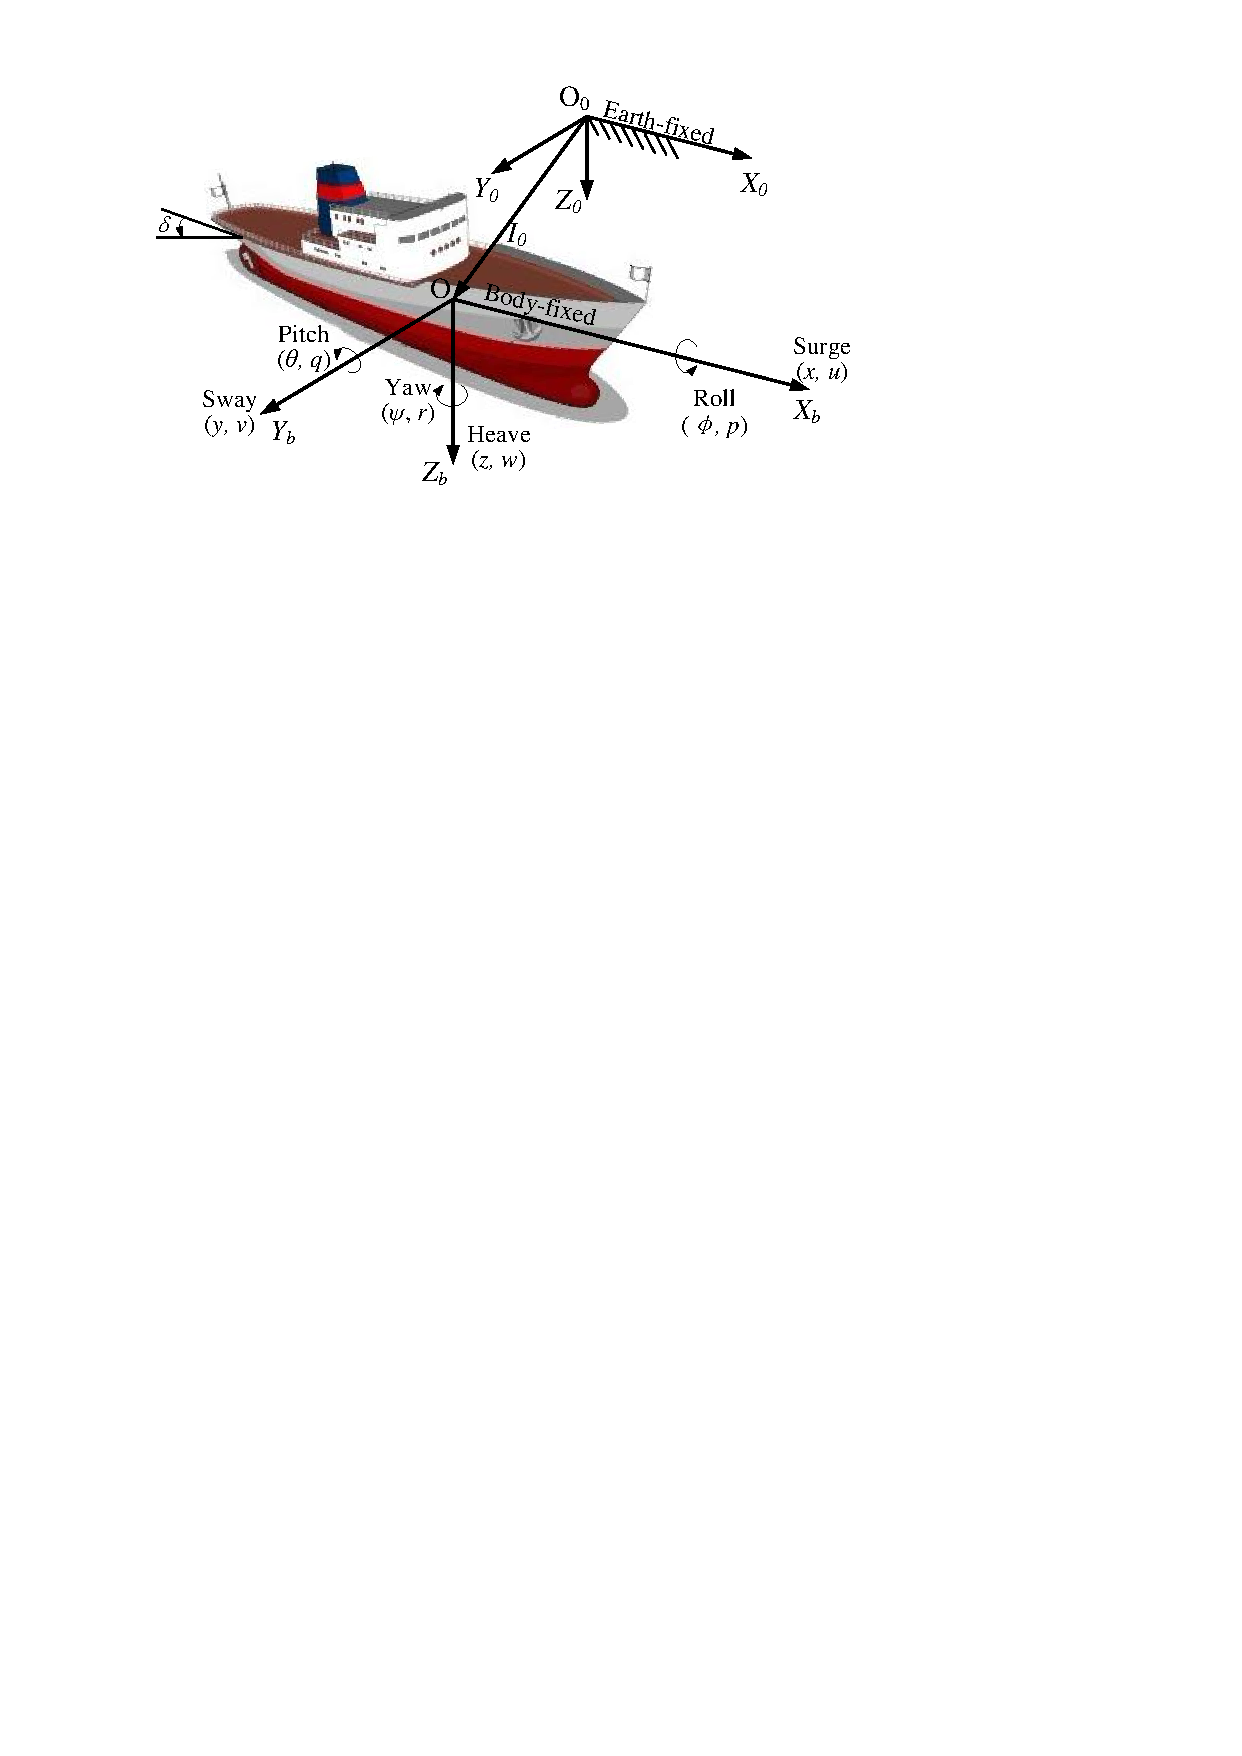
\includegraphics[width=8.5cm]{FIG1_PDF.pdf}%bb=0 0 100 107
\caption{Ship motion in 6-DOF}
\label{FIG1_PDF}
\end{figure}

\newpage

\begin{figure*}[htbp]
\centering
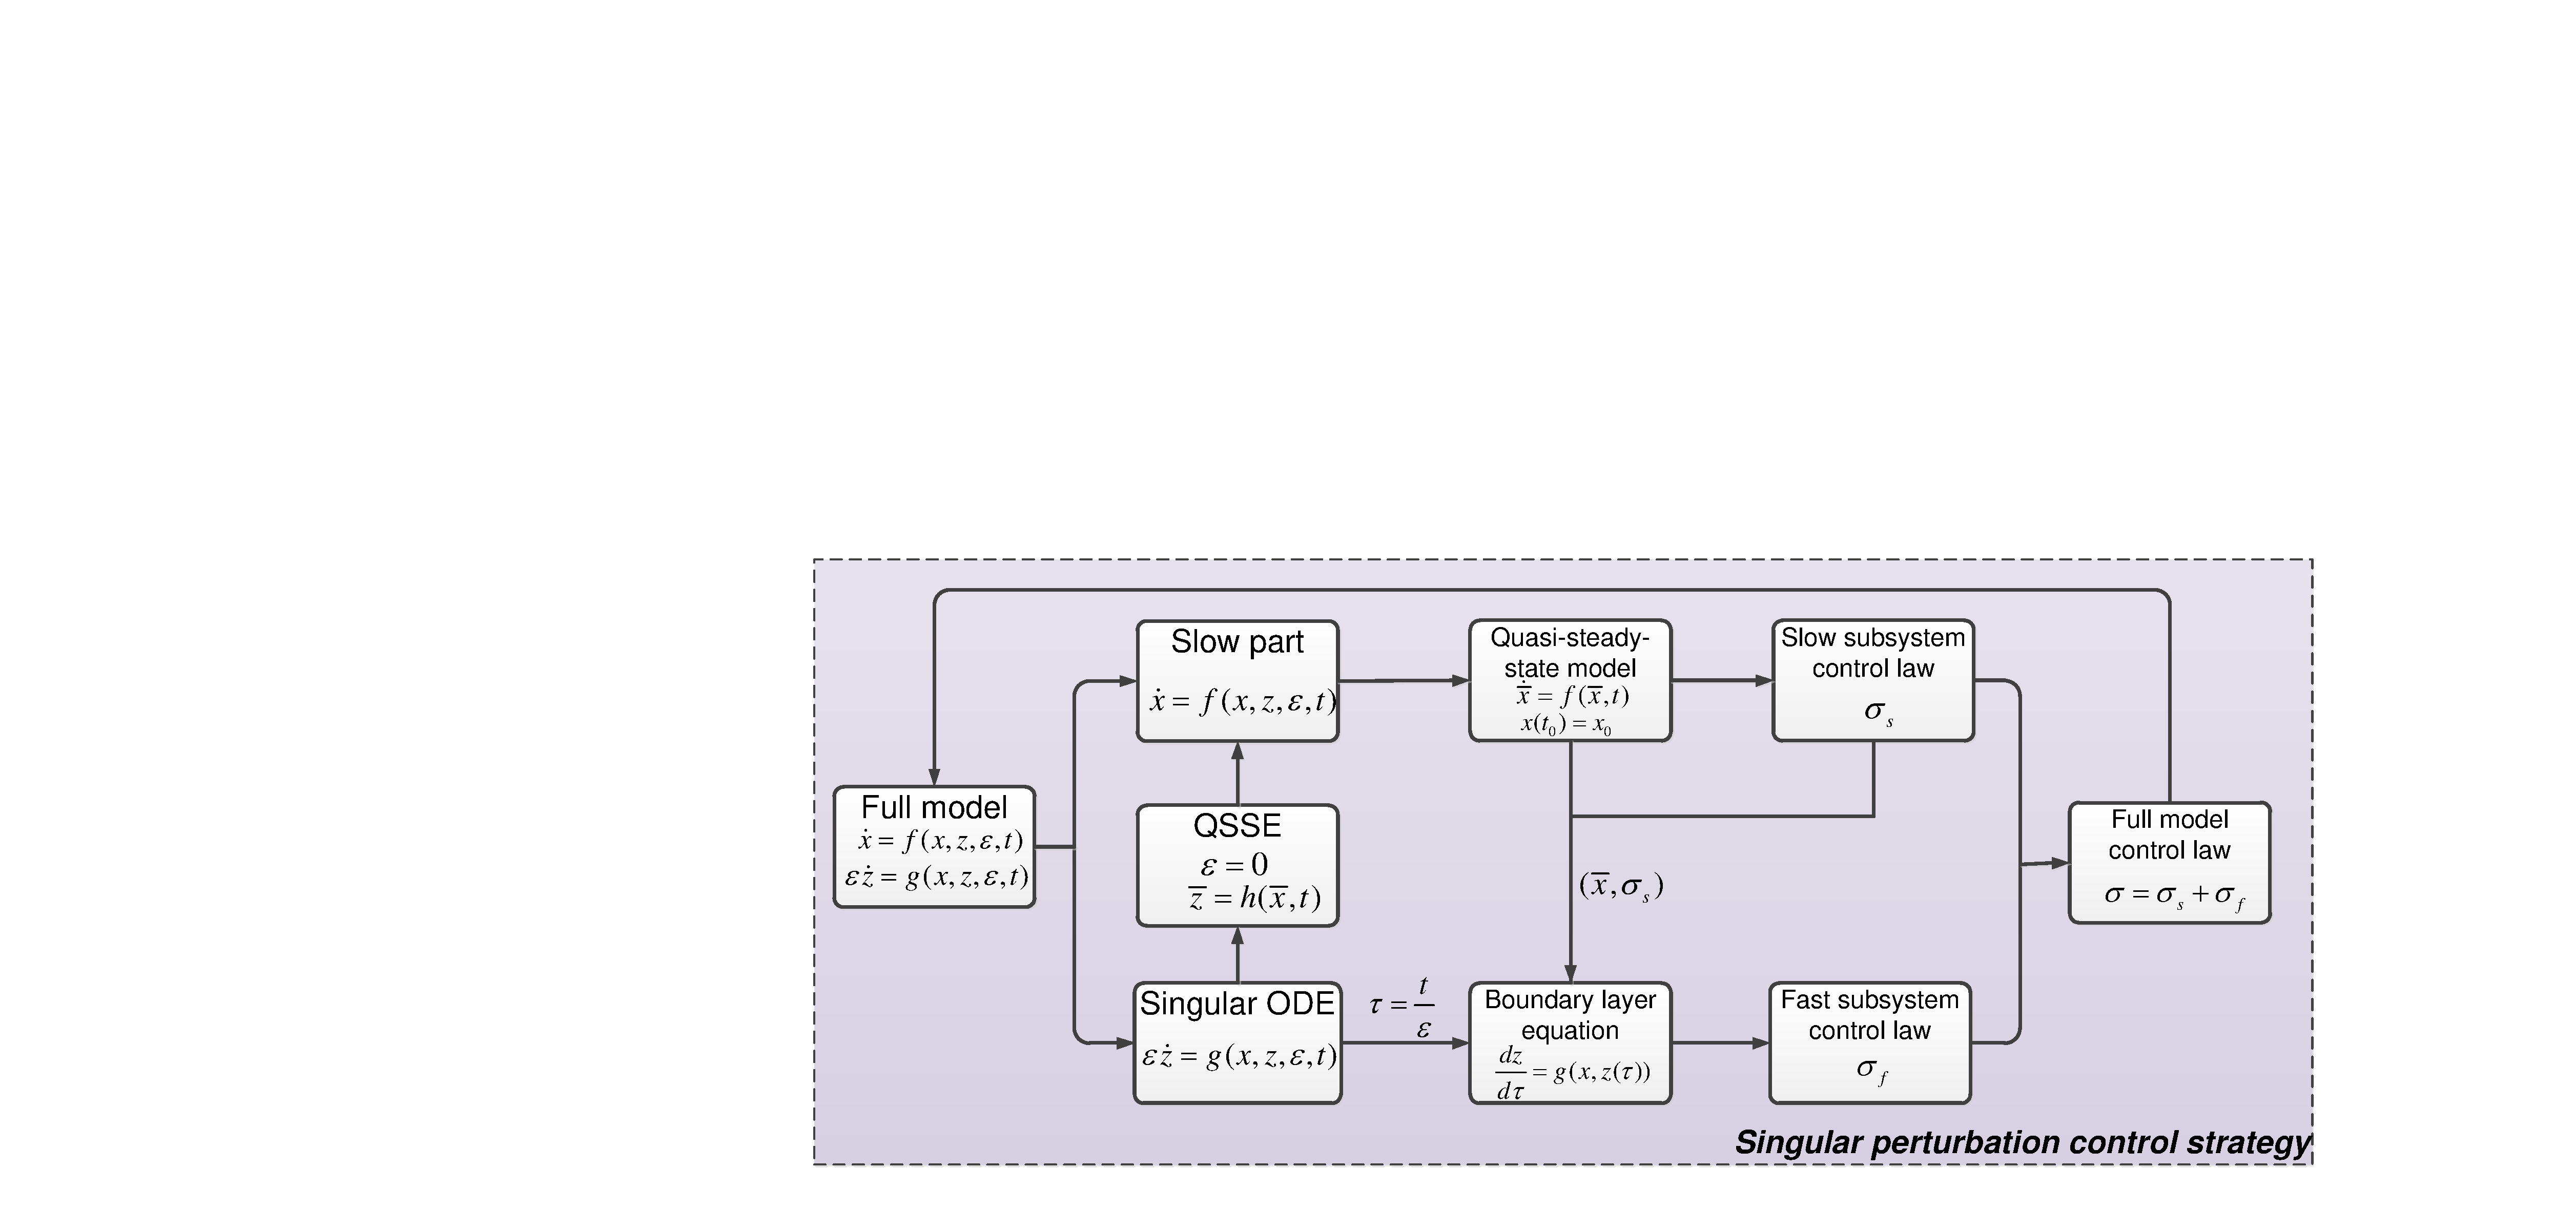
\includegraphics[width=14cm]{FIG2_PDF.pdf}%bb=0 0 100 107
\caption{Singular perturbation control scheme}
\label{FIG2_PDF}
\end{figure*}

\newpage

\begin{figure}[htp]
\centering
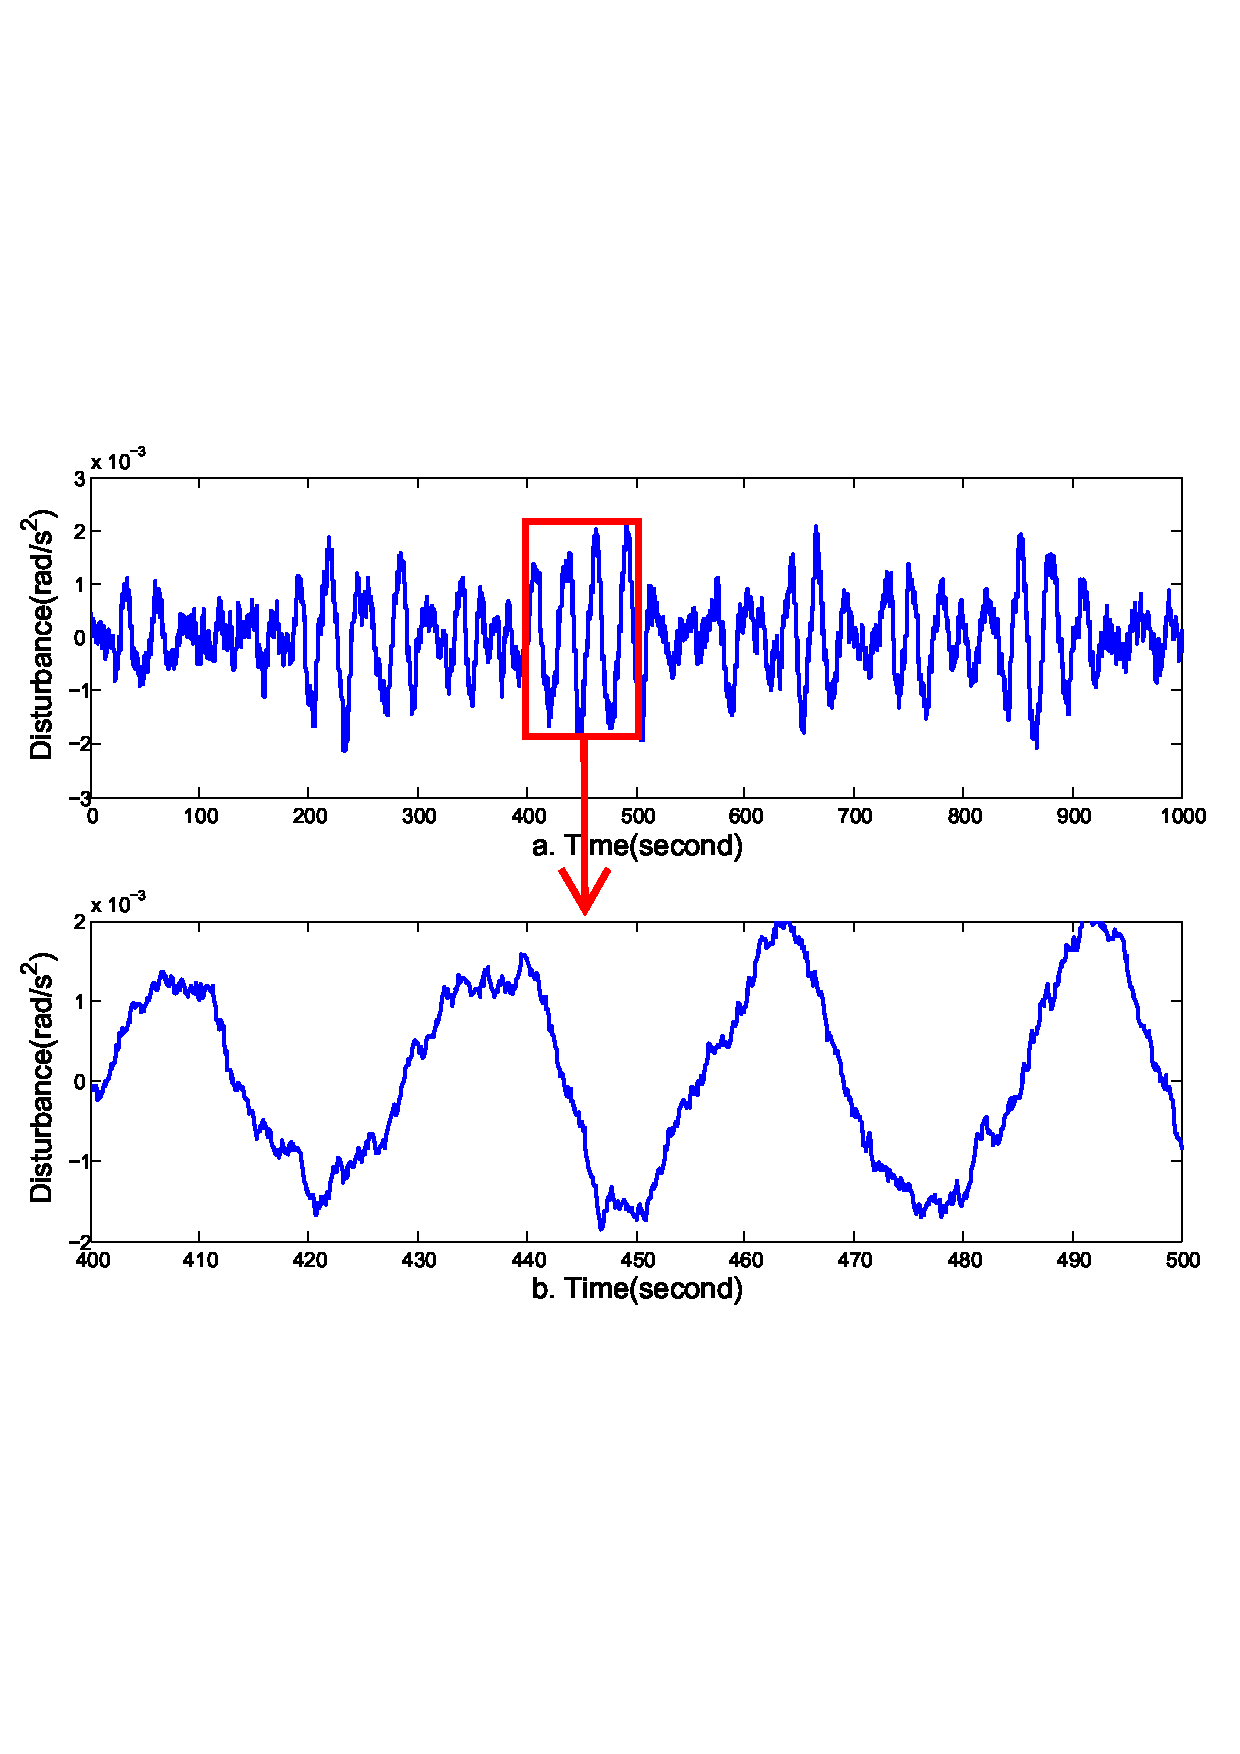
\includegraphics[width=8cm]{FIG3_PDF.pdf}%bb=0 0 100 107
\caption{Wave disturbances of the roll motion, the shaping function parameters are selected as: $K_w=8\times10^{-4}, \xi_0=0.075, \omega_0=0.21$}
\label{FIG3_PDF}
\end{figure}

\newpage

\begin{figure}[htp]
\centering
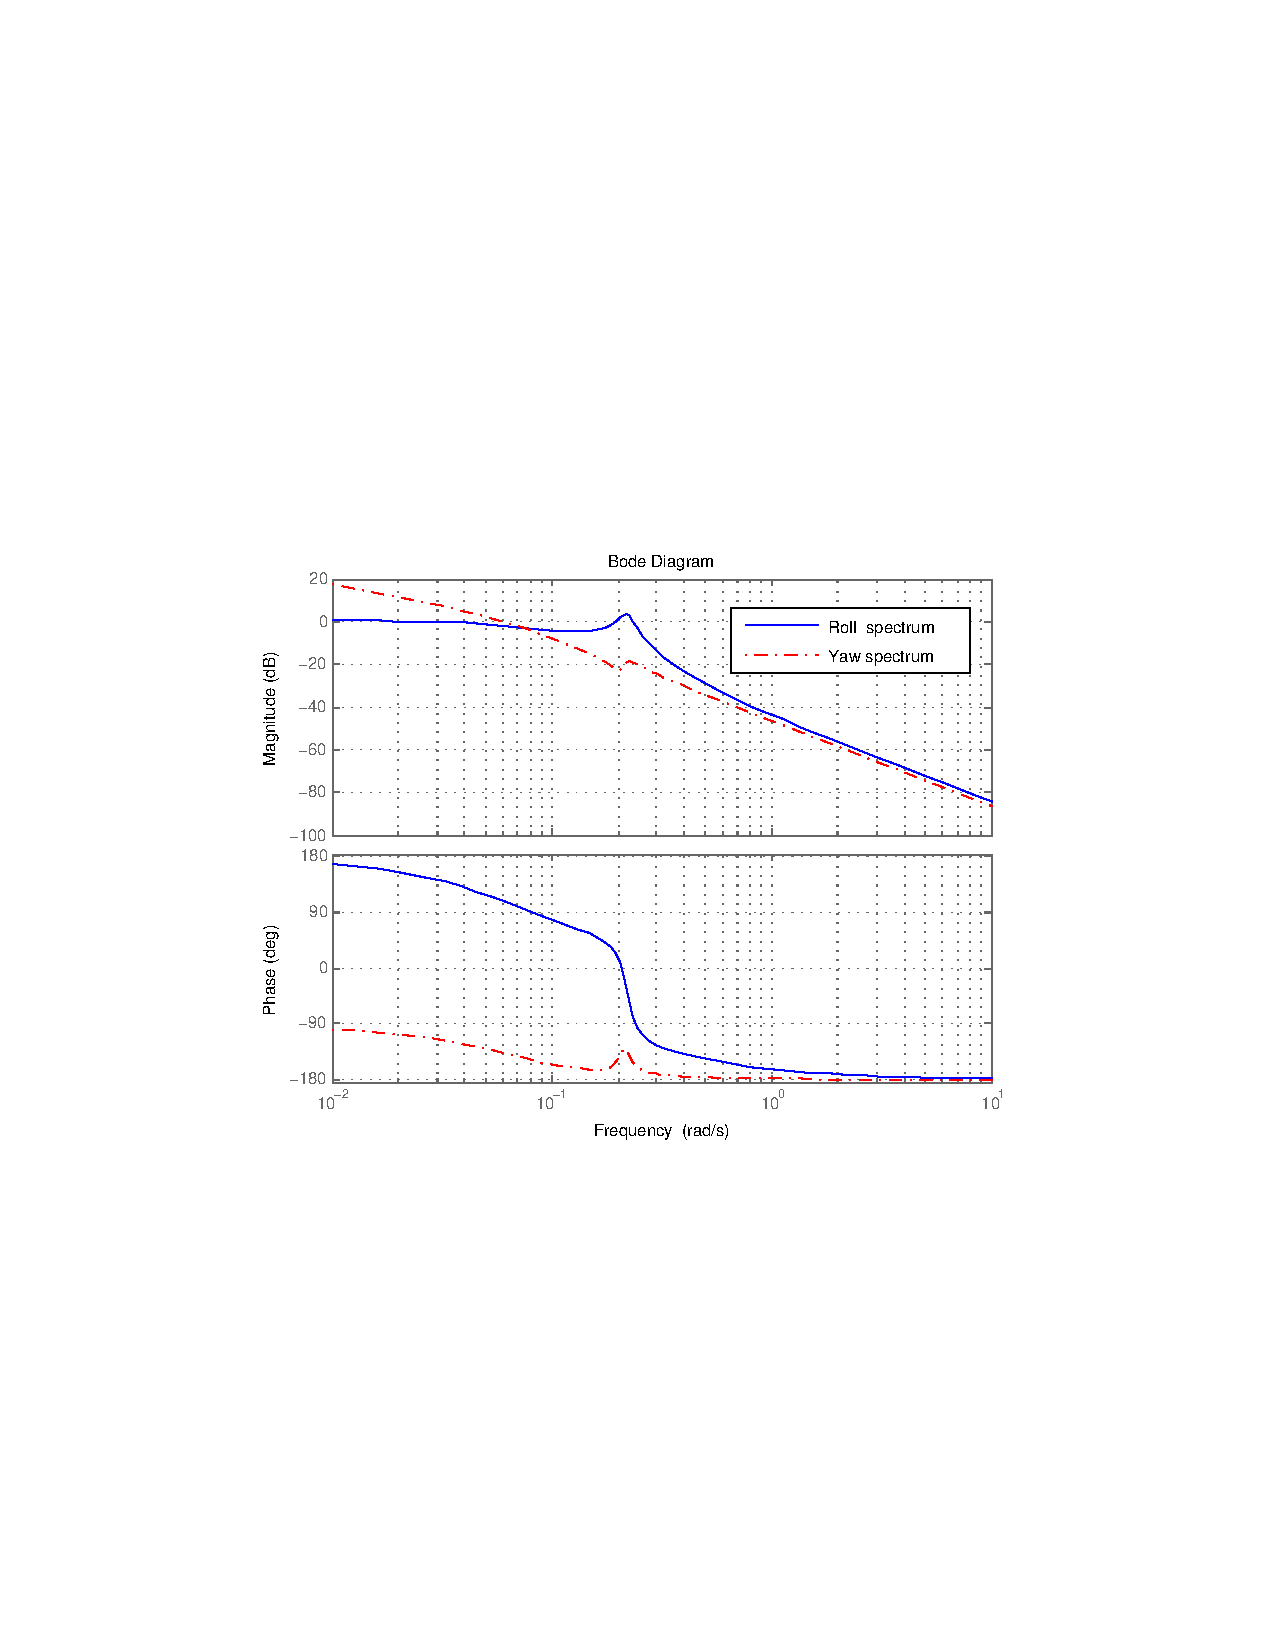
\includegraphics[width=8cm]{FIG4_PDF.pdf}%bb=0 0 100 107
\caption{Bode diagram of yaw spectrum and roll spectrum}
\label{FIG4_PDF}
\end{figure}
\newpage
%
%
%\begin{figure}[htp]
%\centering
%\includegraphics[width=7.5cm]{nonminimum_phenomenon.pdf}%bb=0 0 100 107
%\caption{nonminimum phase phenomenon }
%\label{fig:3}
%\end{figure}
%
%
%


\begin{figure}[htp]
\centering
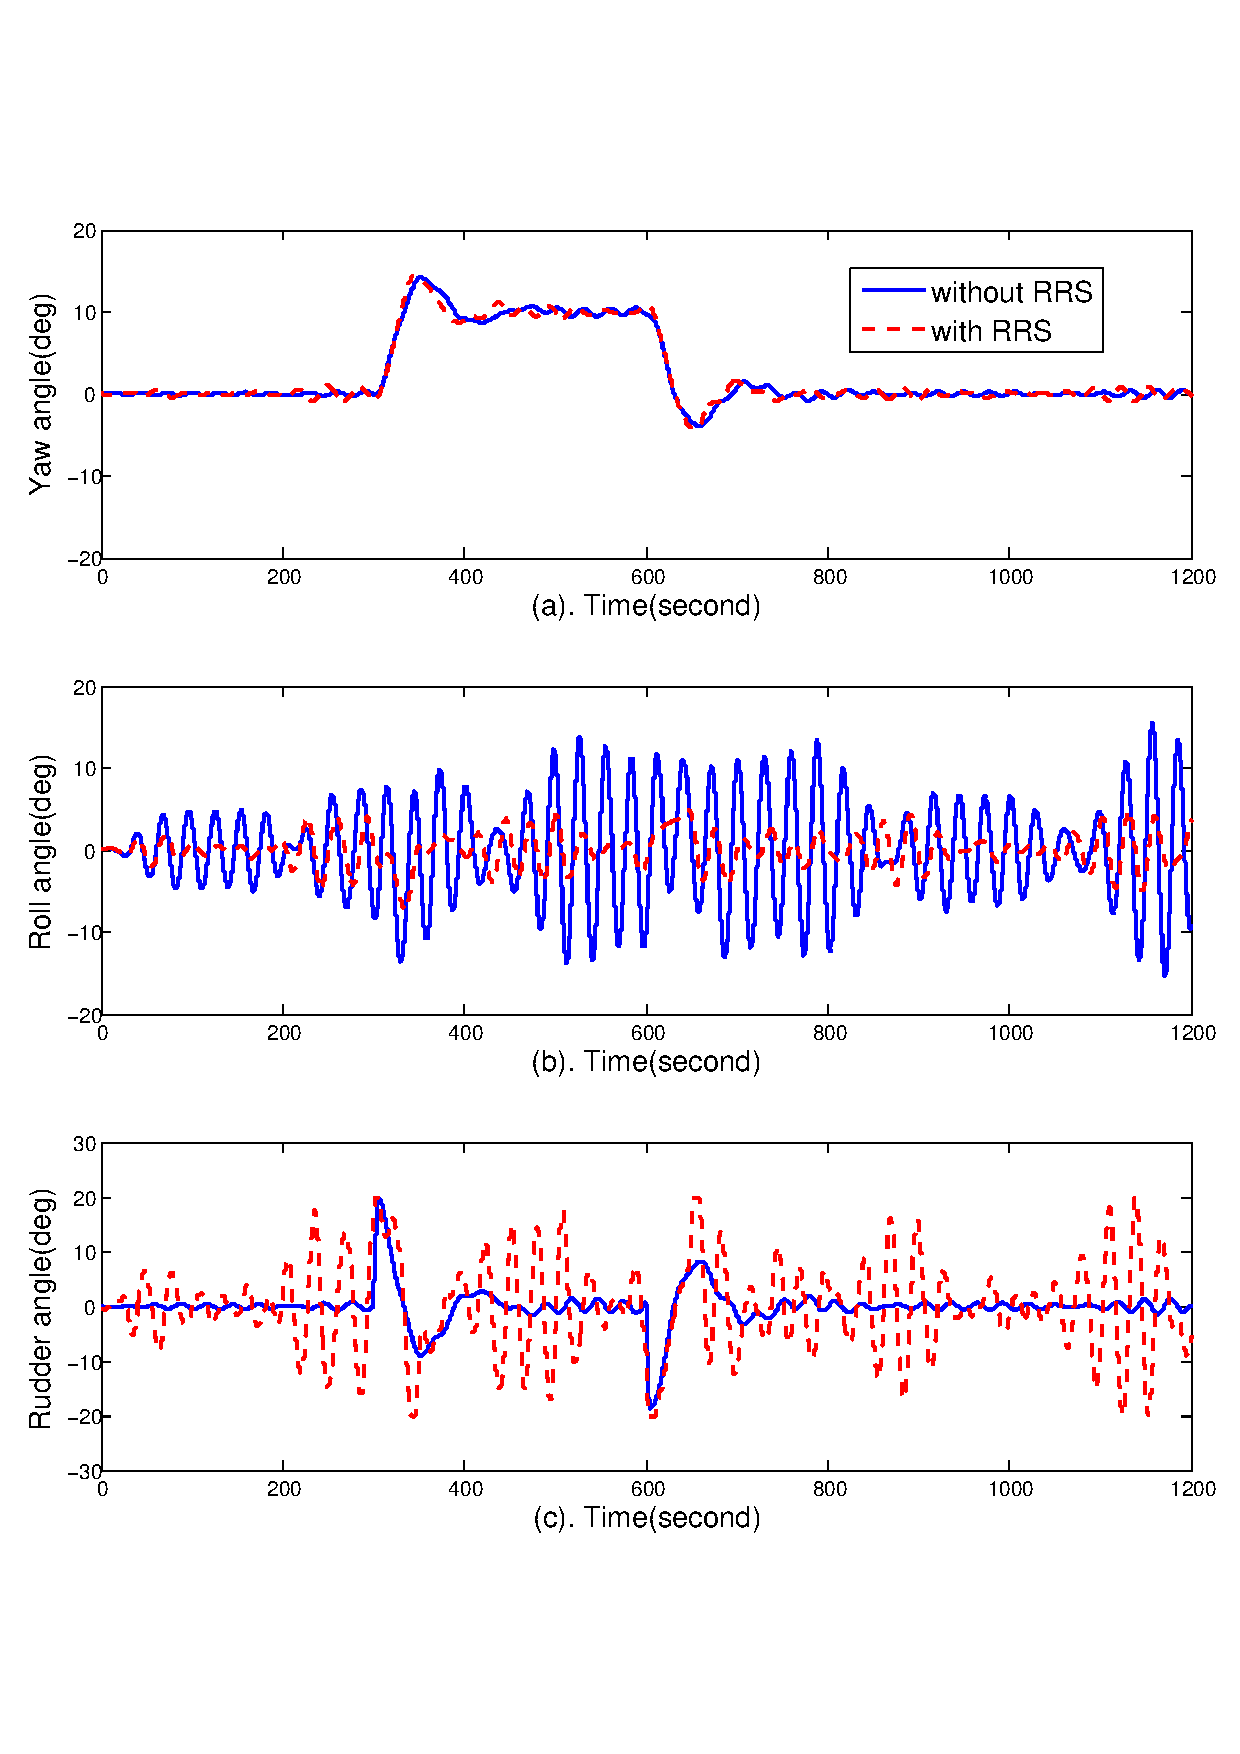
\includegraphics[width=8cm]{FIG5_PDF.pdf}%bb=0 0 100 107
\caption{Nonlinear model simulation results with and without RRS: (a) yaw angle, (b) roll angle and (c) rudder angle.}
\label{FIG5_PDF}
\end{figure}

\newpage


\begin{figure}[htp]
\centering
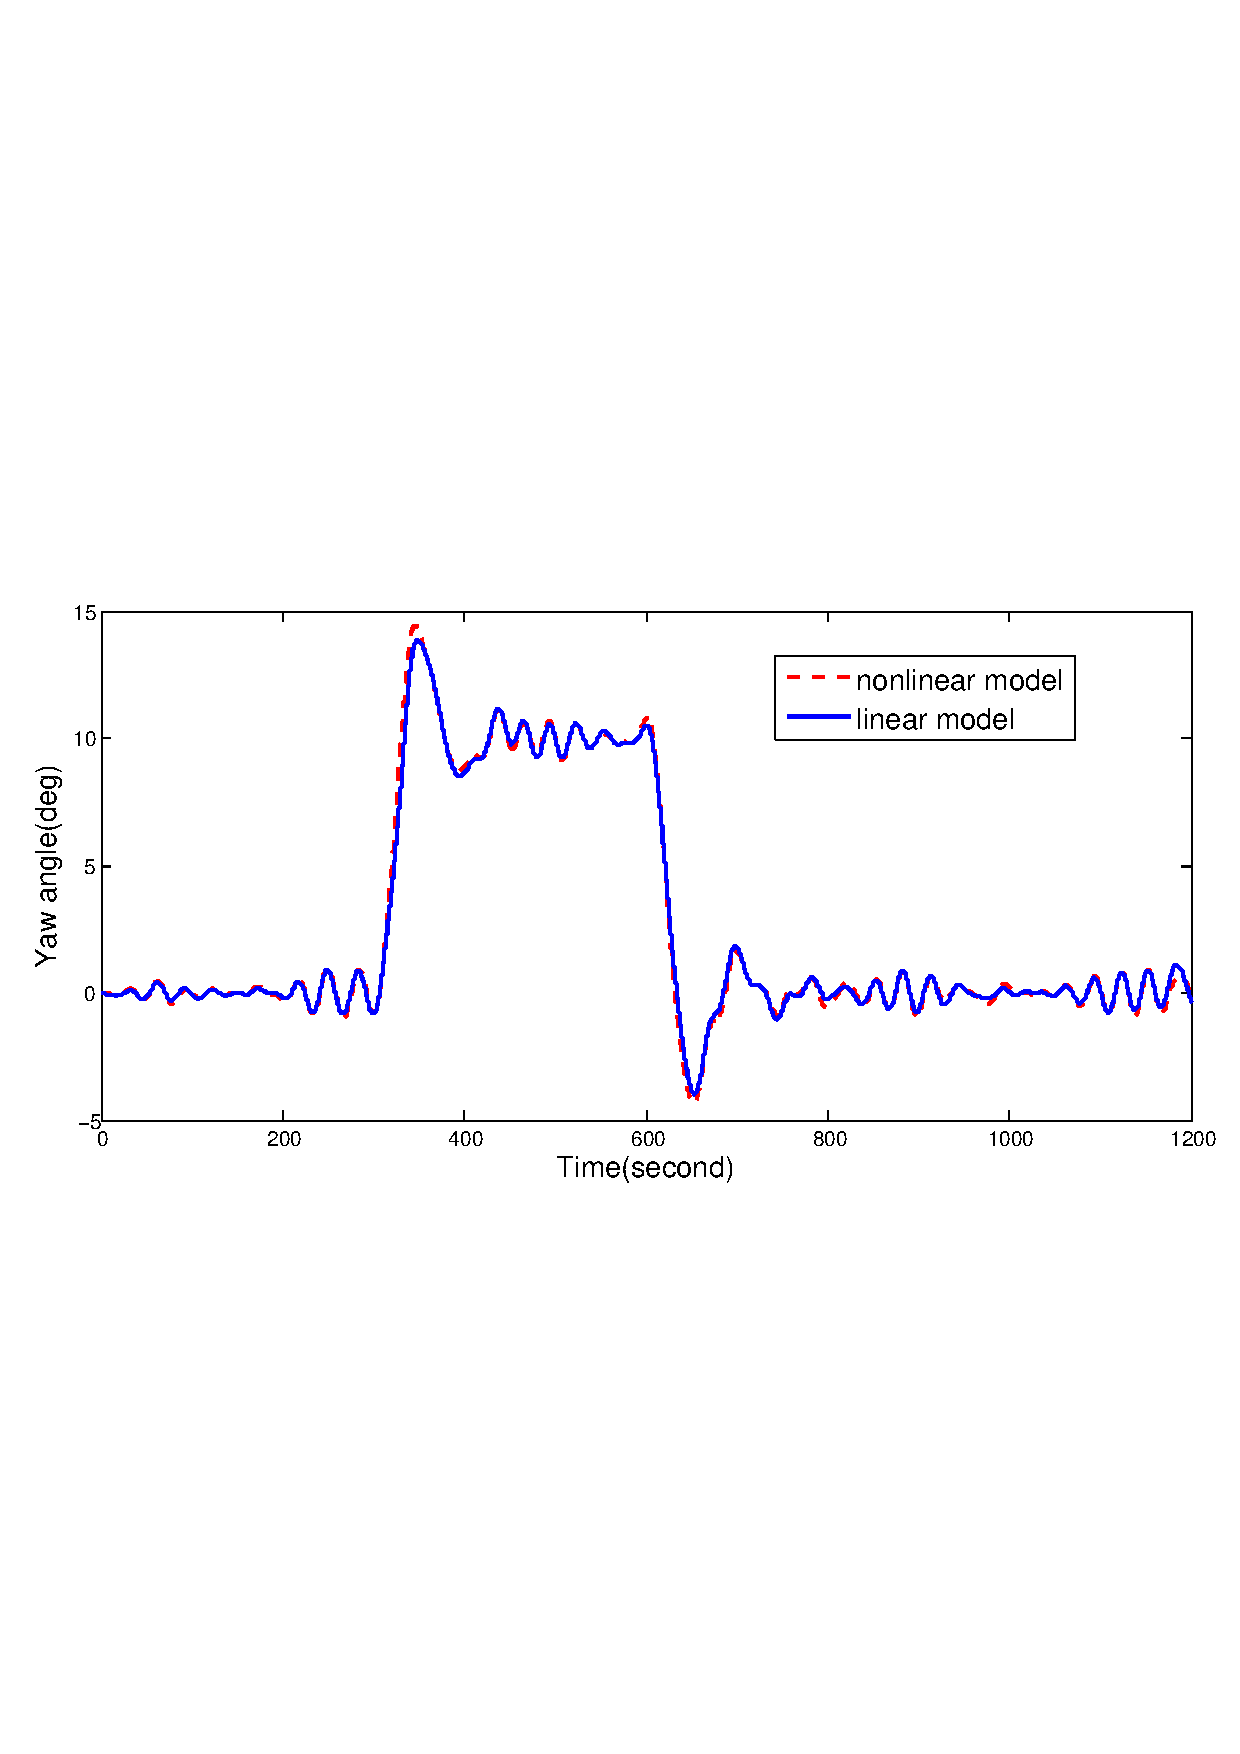
\includegraphics[width=8cm]{FIG6_PDF.pdf}%bb=0 0 100 107
\caption{Yaw angle performances of the linear and nonlinear models with RRS control strategy.}
\label{FIG6_PDF}
\end{figure}

\newpage

\begin{figure}[htp]
\centering
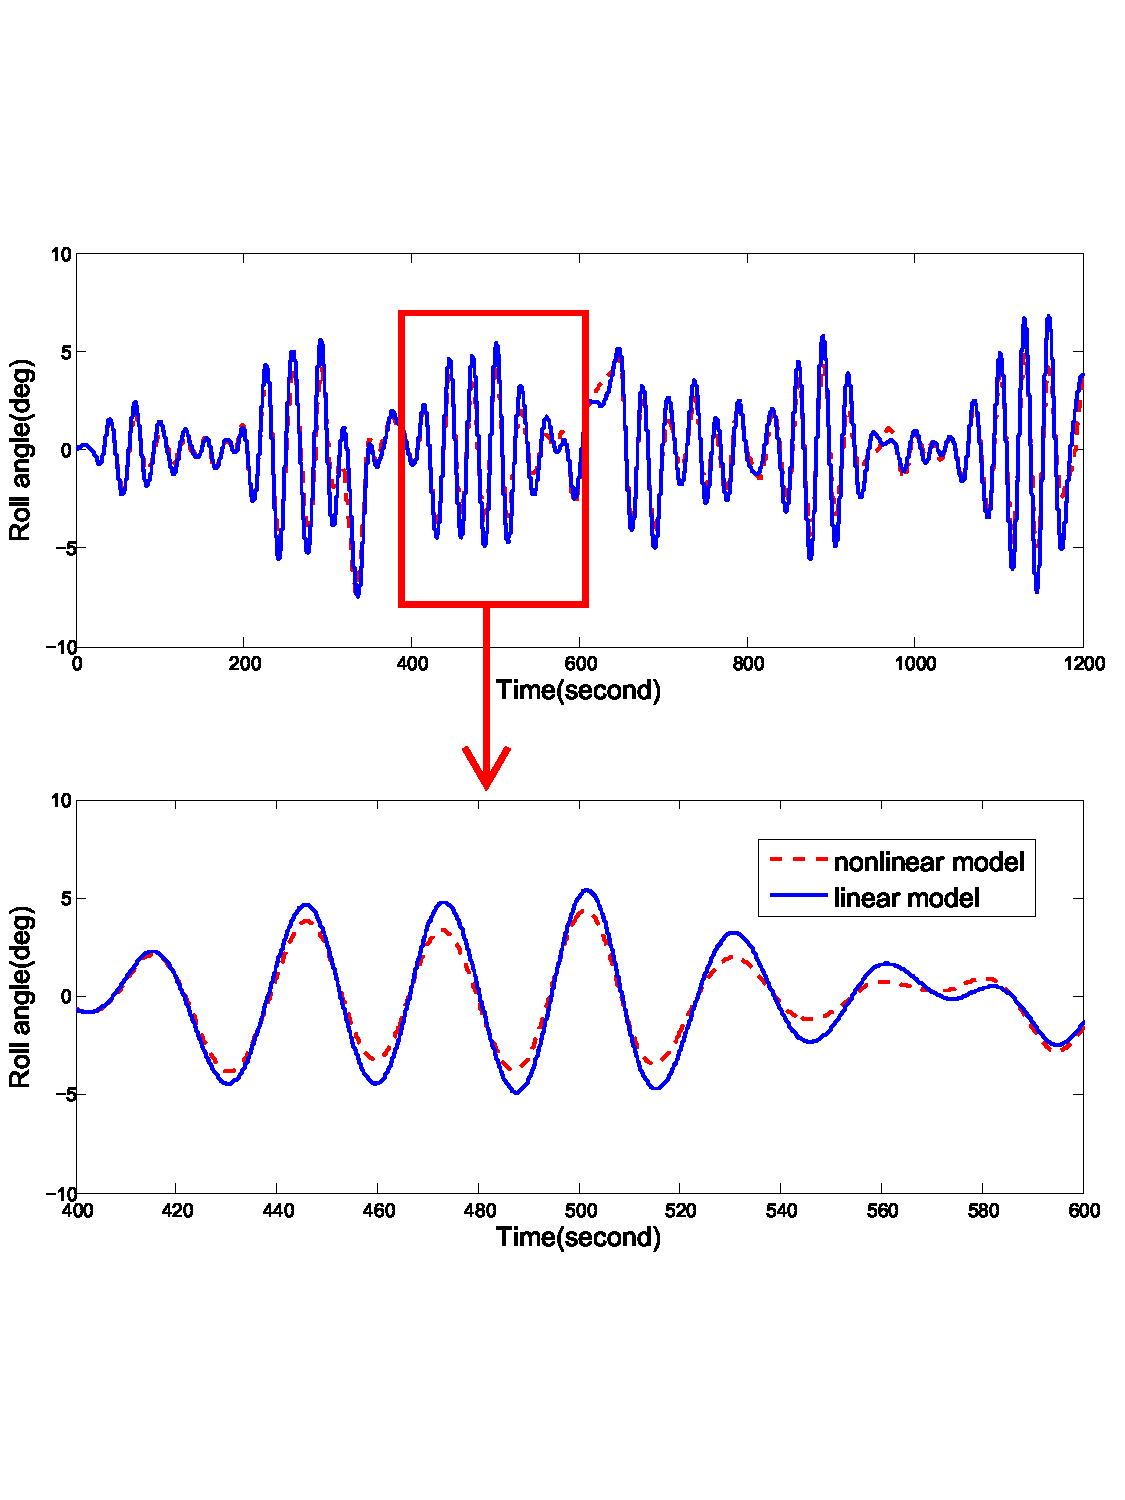
\includegraphics[width=8cm]{FIG7_PDF.pdf}%bb=0 0 100 107
\caption{Roll angle performances of the linear and nonlinear models with RRS control strategy.}
\label{FIG7_PDF}
\end{figure}

\newpage

\begin{figure}[htbp]
\centering
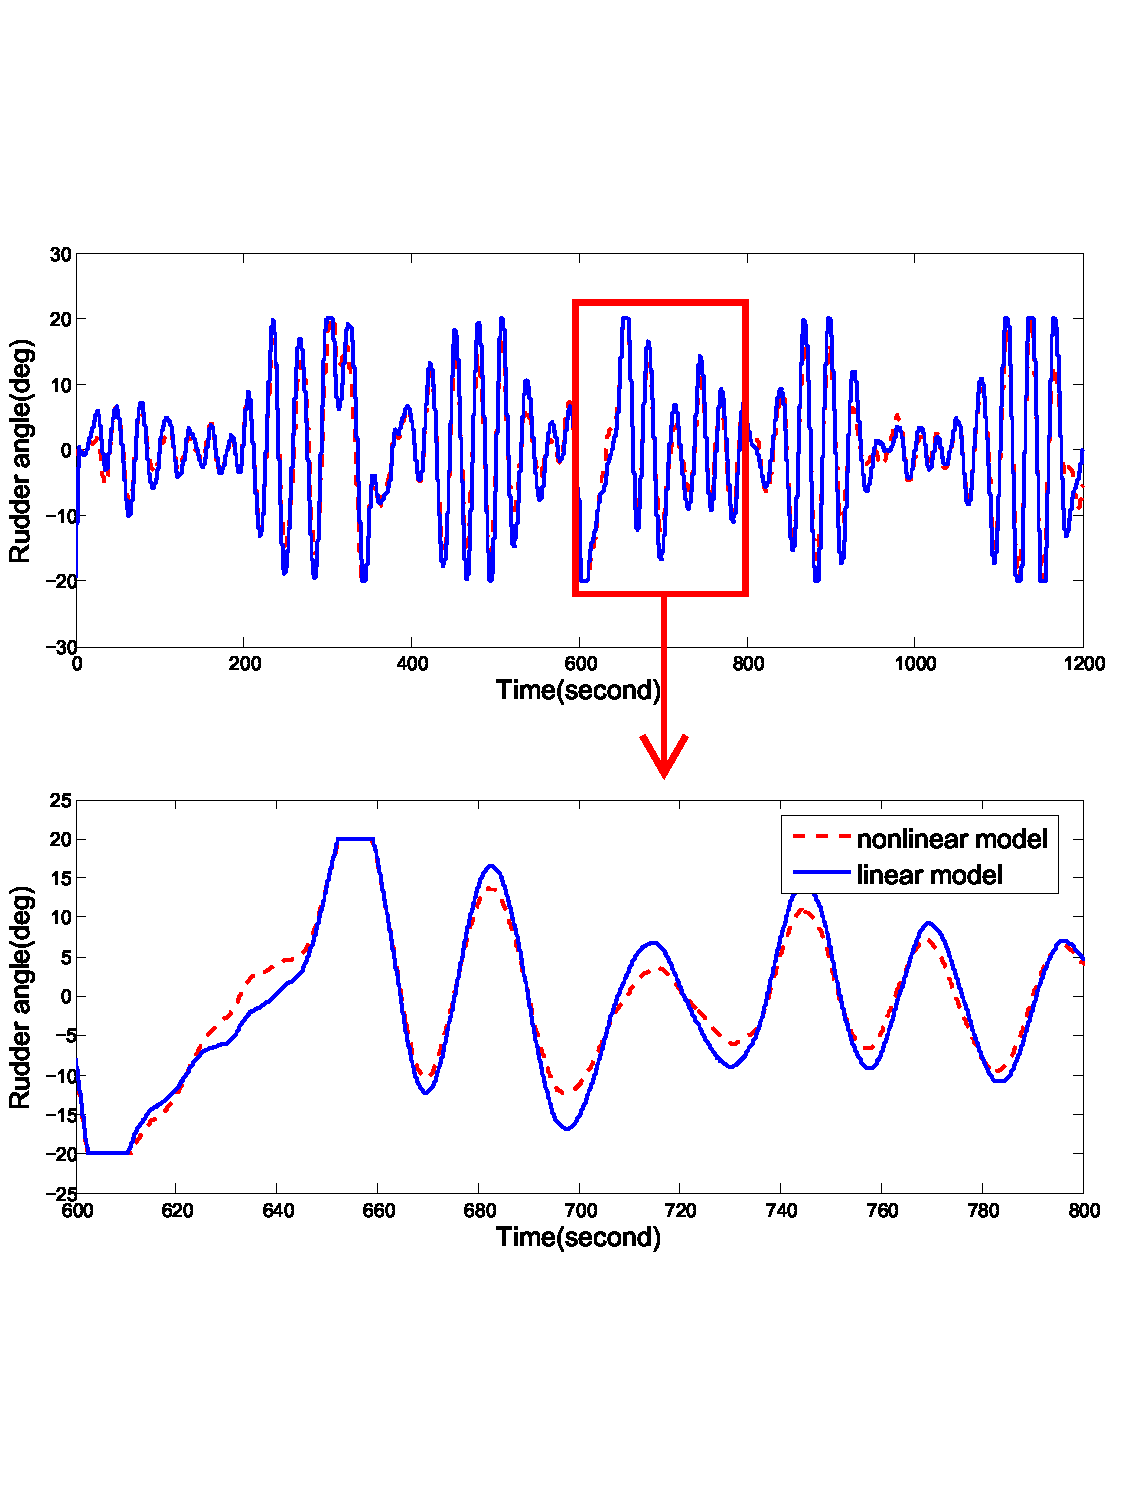
\includegraphics[width=8cm]{FIG8_PDF.pdf}%bb=0 0 100 107
\caption{Rudder angle performances of the linear and nonlinear models with RRS control strategy.}
\label{FIG8_PDF}
\end{figure}



\newpage

\begin{figure}[htp]
\centering
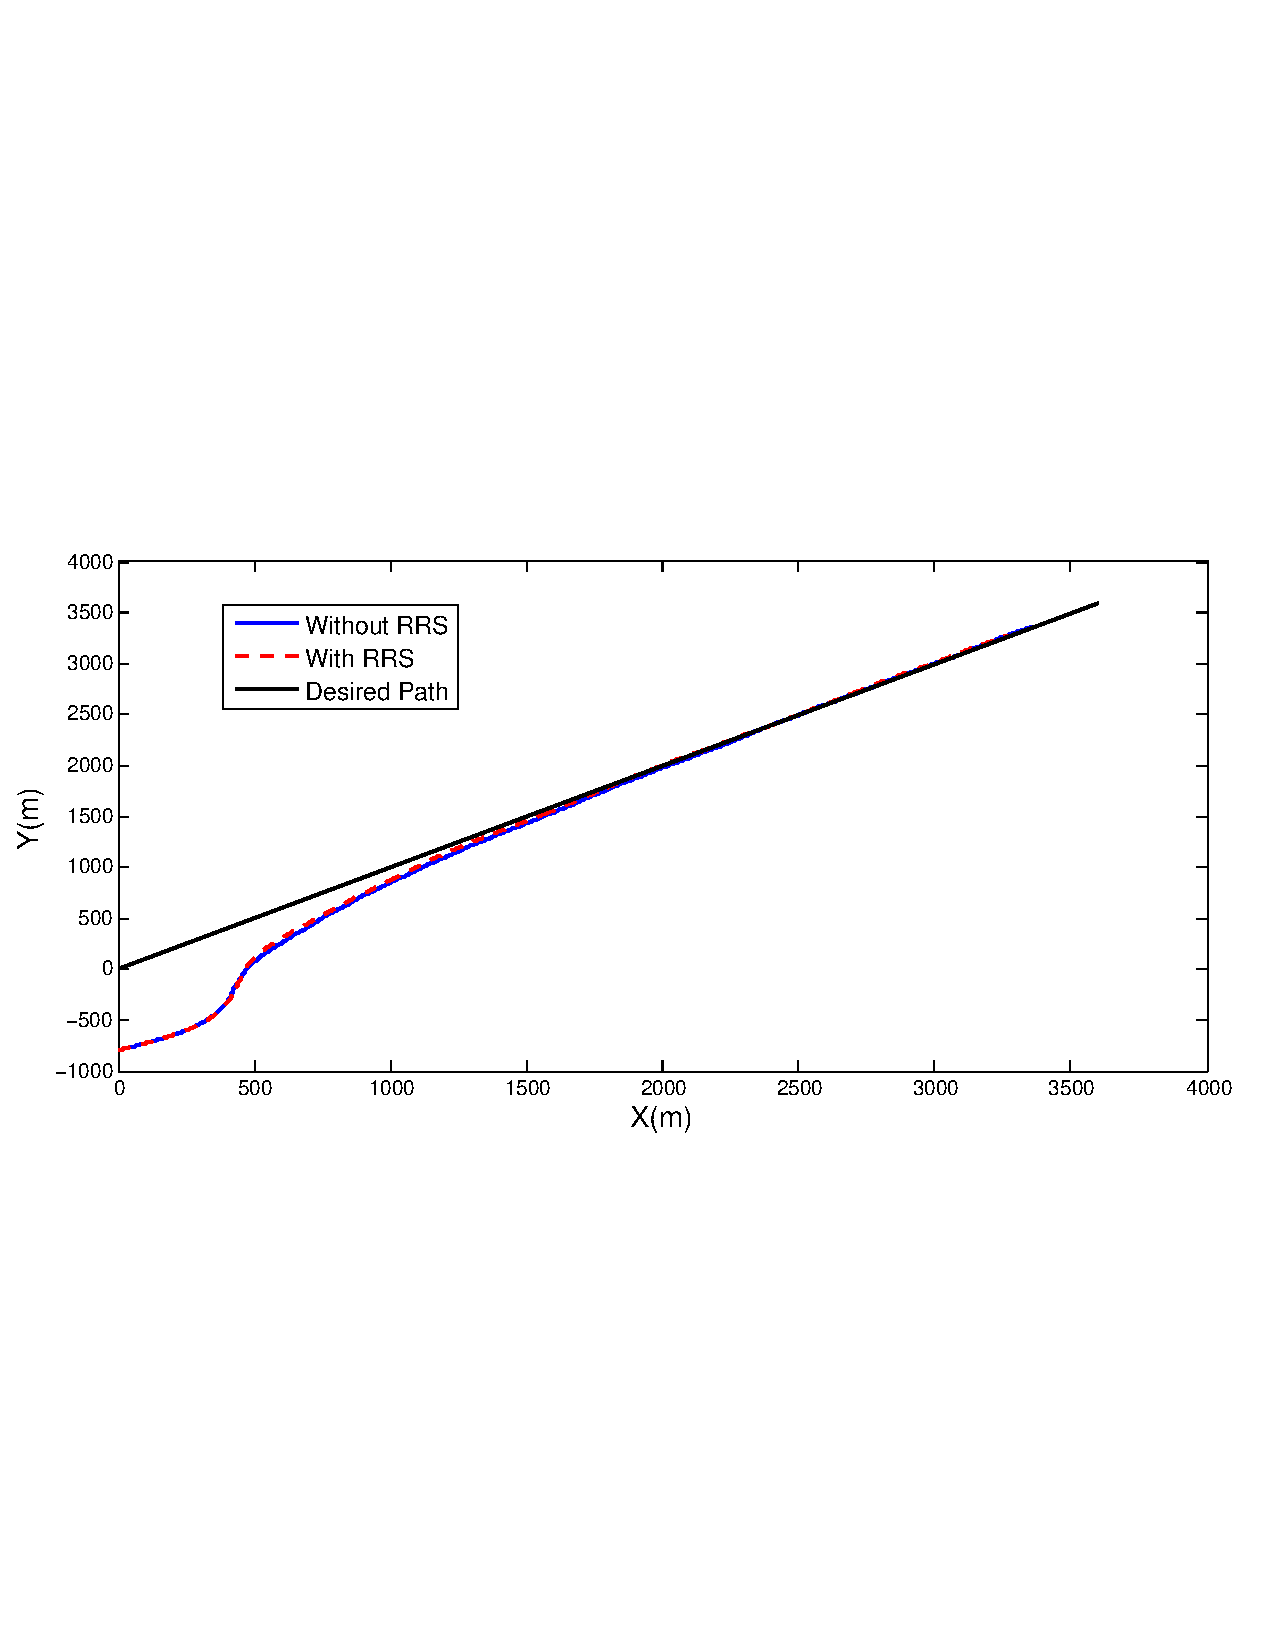
\includegraphics[width=8cm]{FIG10_PDF.pdf}%bb=0 0 100 107
\caption{Track keeping performances with and without RRS control strategy}
\label{FIG10_PDF}
\end{figure}


\newpage

\begin{figure}[htp]
\centering
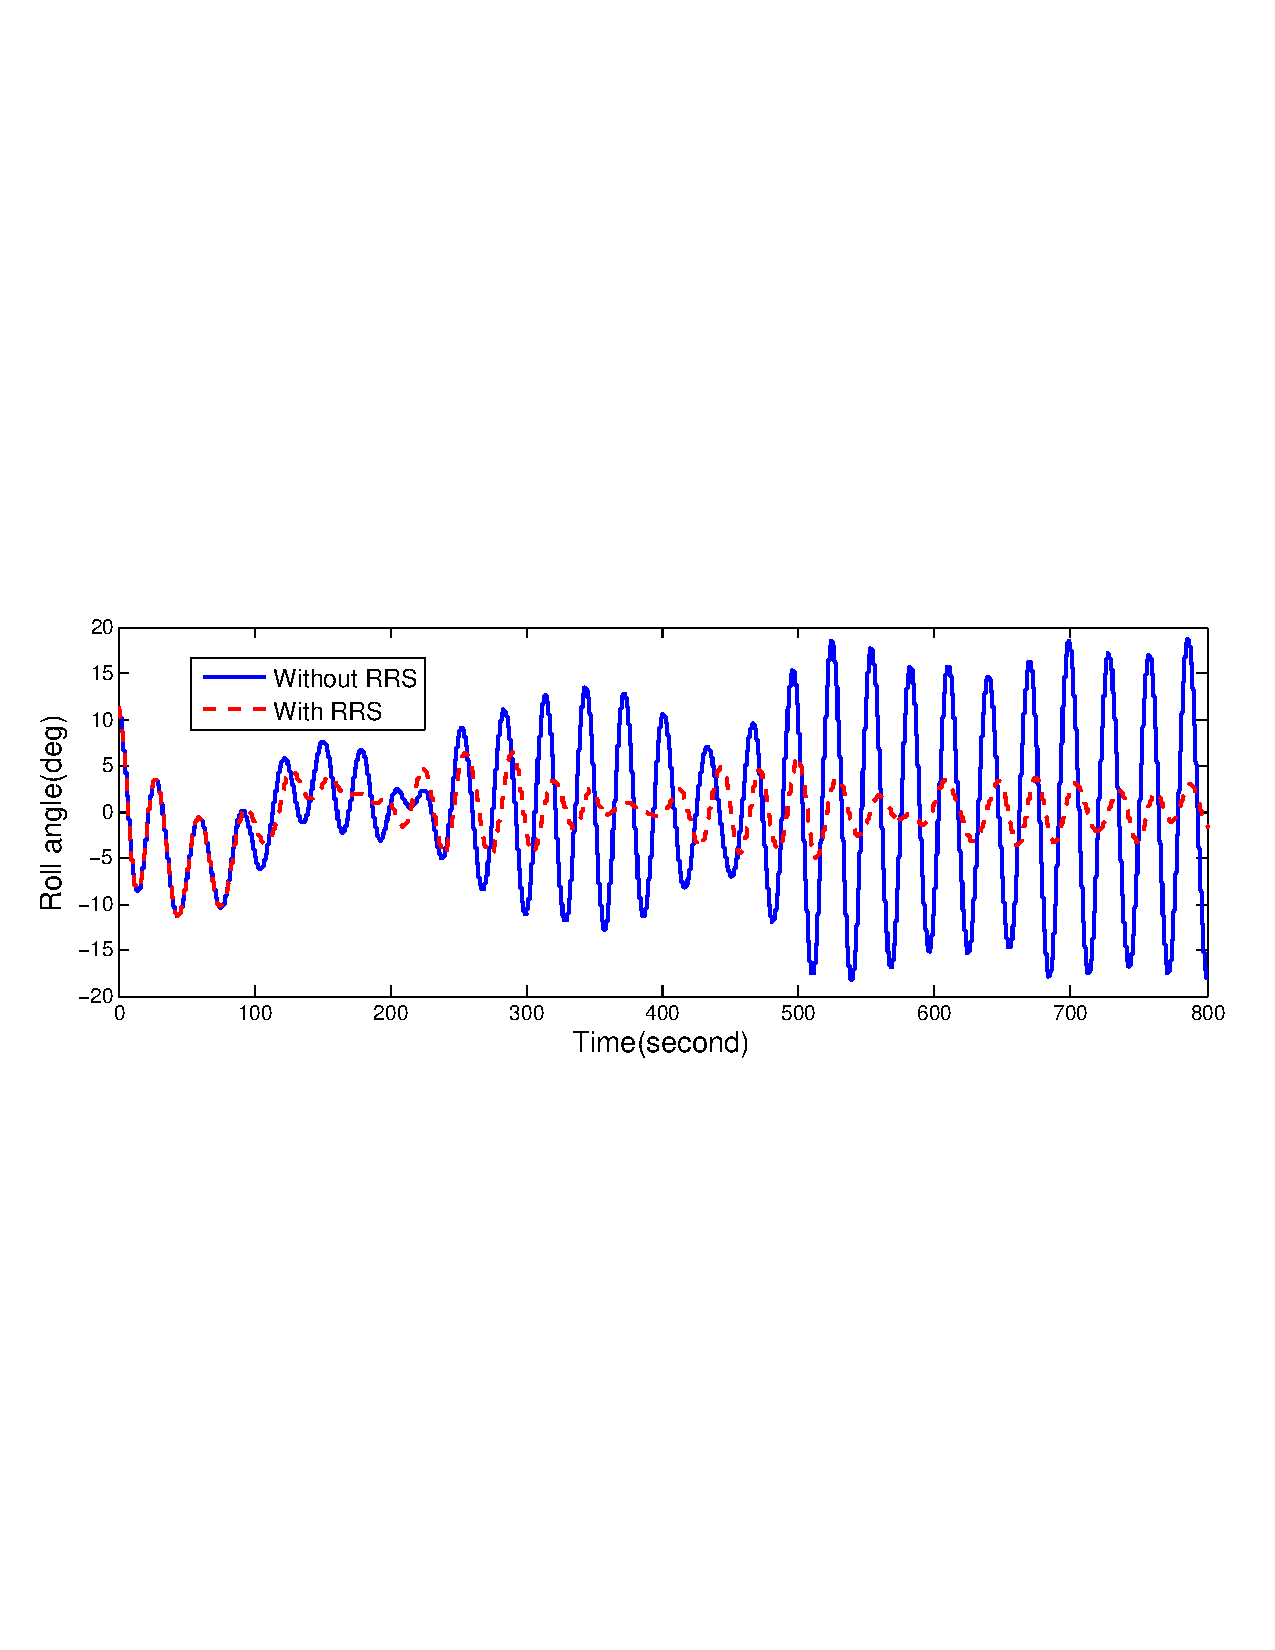
\includegraphics[width=8cm]{FIG11_PDF.pdf}%bb=0 0 100 107
\caption{Roll angle performances in the track keeping operations with and without RRS}
\label{FIG11_PDF}
\end{figure}





\newpage

\begin{figure}[htp]
\centering
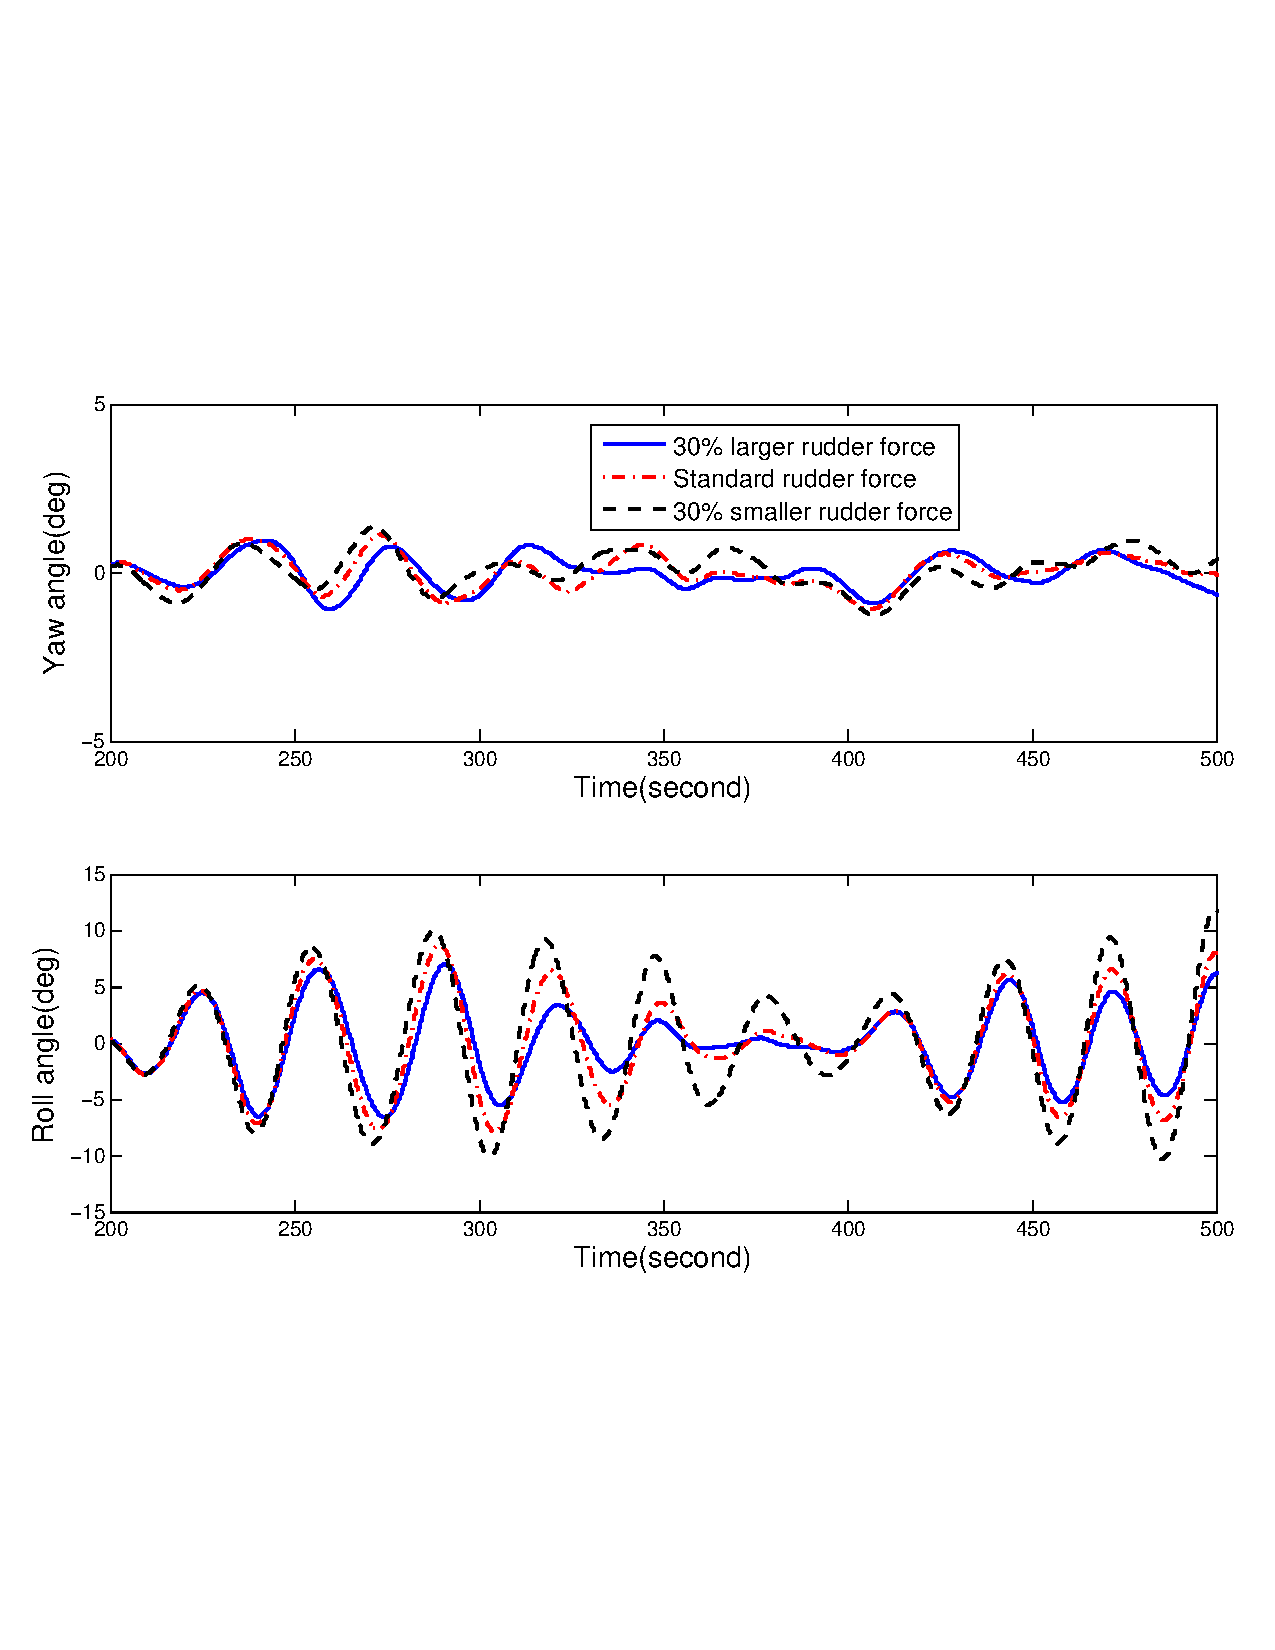
\includegraphics[width=8cm]{FIG9_PDF.pdf}%bb=0 0 100 107
\caption{Sensitivity analysis of rudder model errors}
\label{FIG9_PDF}
\end{figure}


% \bibitem{}

% \end{thebibliography}


\end{document}

%%
%% End of file `elsarticle-template-1b-num.tex'.
